\documentclass[beamer=true]{standalone}
\usepackage{../../preamblesnotes}

%Information to be included in the title page:
\title{第二課}
\author{力和運動Force and motion}
\institute{全年班}
\date{}

\begin{document}
\frame{\titlepage}

\begin{frame}{力的性質Properties of forces}
    \begin{itemize}
        \item 可分為接觸力和非接觸力。\\Forces can be categorised into contact forces and non-contact forces.
              \begin{itemize}
                  \item 接觸力:包括張力、法向力、摩擦力、流體阻力;\\Contact forces: includes tensions, normal forces, frictions and fluid resistances;
                  \item 接觸力:包括張力、法向力、摩擦力、流體阻力;\\Contact forces: includes tensions, normal forces, frictions and fluid resistances;
                  \item 非接觸力:包括重量、電力、磁力。\\non-contact forces: includes gravitational force, electric forces, and magnetic forces.
              \end{itemize}
        \item 在國際單位制中,力的單位是牛頓,符號為\textbf{N}。\\The S.I. unit of forces is Newton, which can be written as \textbf{N}.

    \end{itemize}
\end{frame}

\begin{frame}{力的性質Properties of forces}
    \begin{itemize}
        \item 力是矢量,有量值和方向。向某方向作用的力,可用箭號來表示,箭號的方向和長度分別顯示力的方向和量值。 \\Forces are vectors consisting of magnitudes and directions and represented by arrows. The directions and magnitudes of the arrows represent that of the forces.
              % \item 在實驗室裏,通常使用彈簧秤或感應器去量度力的大小。彈簧秤只能量度拉力,而接駁數據記錄器的力感應器則可以量度拉力和推力。 \\In laboratories, it is common to use spring balance to measure forces. However, spring balances can only measure pulling forces, while a force sensor connected to a datalogger measures both pulling forces and pushing forces.
    \end{itemize}
\end{frame}

\begin{frame}{重量 (W) Weight (W)}
    \begin{itemize}
        \item 地球作用於物體的拉力。\\Pulling forces acting on objects by the Earth.
        \item 方向指向地球的中心。\\ Its direction is towards the center of Earth.
        \item W=mg, g = 重力加速度acceleration due to gravity
    \end{itemize}
    \begin{columns}
        \column{.5\textwidth}
        \centering
        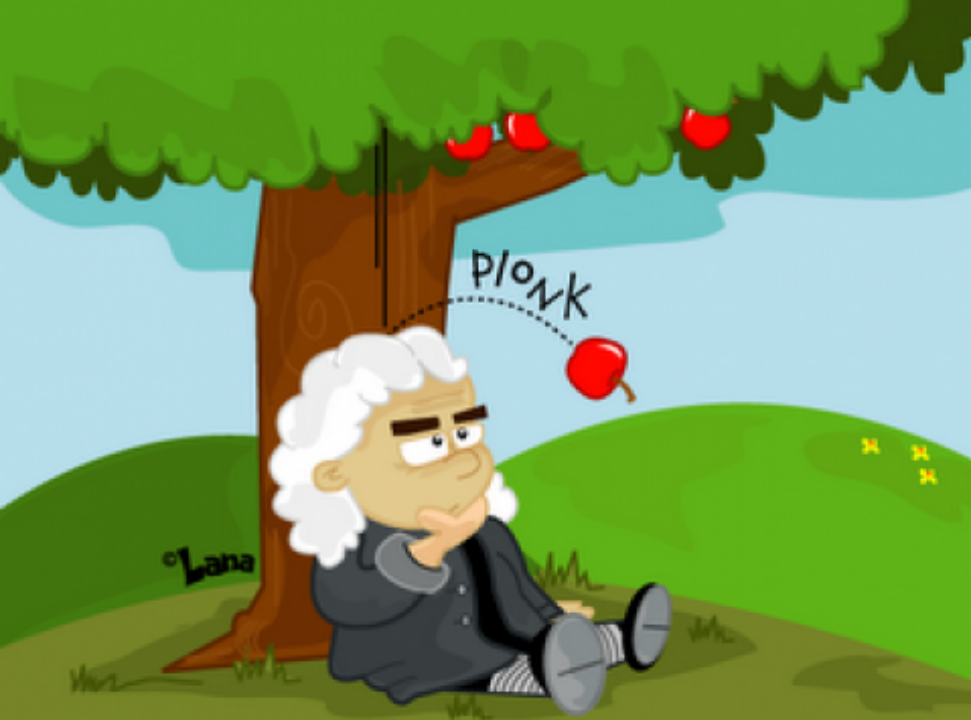
\includegraphics[width=\textwidth]{assets/47712628.png}
        \column{.5\textwidth}
        \begin{figure}[h!]
            \centering
            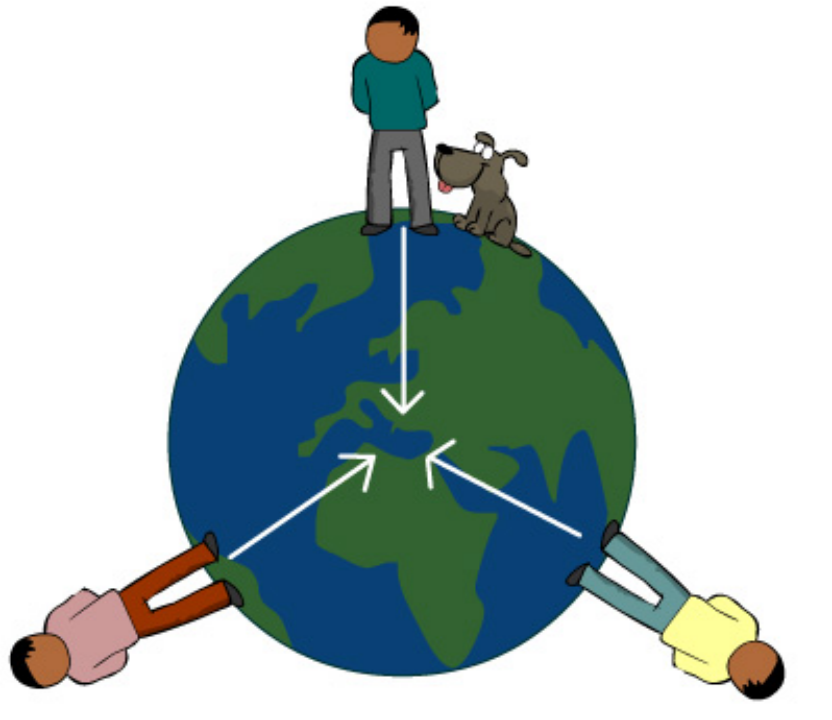
\includegraphics[width=\textwidth]{assets/97f12fb9.png}
        \end{figure}
    \end{columns}


\end{frame}


\begin{frame}{張力(T) Tension(T)}
    \begin{itemize}
        \item 繩子拉緊時產生的力。\\Forces generated when a string is pulled tightly.
        \item 在無質量的繩子裏,繩子每一點的張力量值都是相同的。\\In a massless rope, the tension at every point of the rope is the same.
    \end{itemize}
    \begin{figure}[h!]
        \centering
        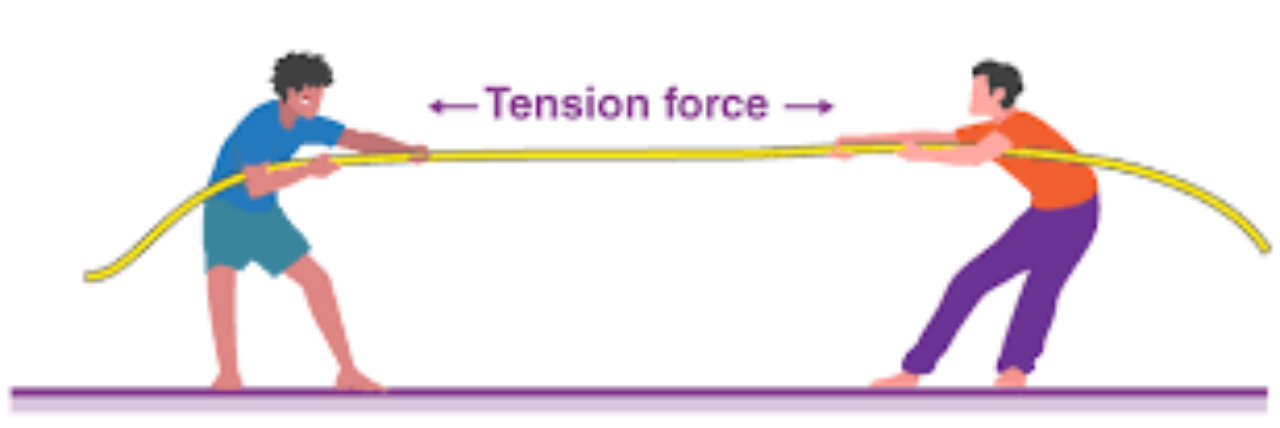
\includegraphics[width=0.66\textwidth]{assets/5673f702.png}
    \end{figure}
\end{frame}

\begin{frame}{法向力 (N 或 R) Normal force (N or R)}
    \begin{itemize}
        \item 兩個物件的表面接觸所產生的力。\\Forces generated between two contact forces.
        \item 力和表面必定互相垂直。\\Force and surface are always perpendicular to each other.
    \end{itemize}
    \begin{figure}[h!]
        \centering
        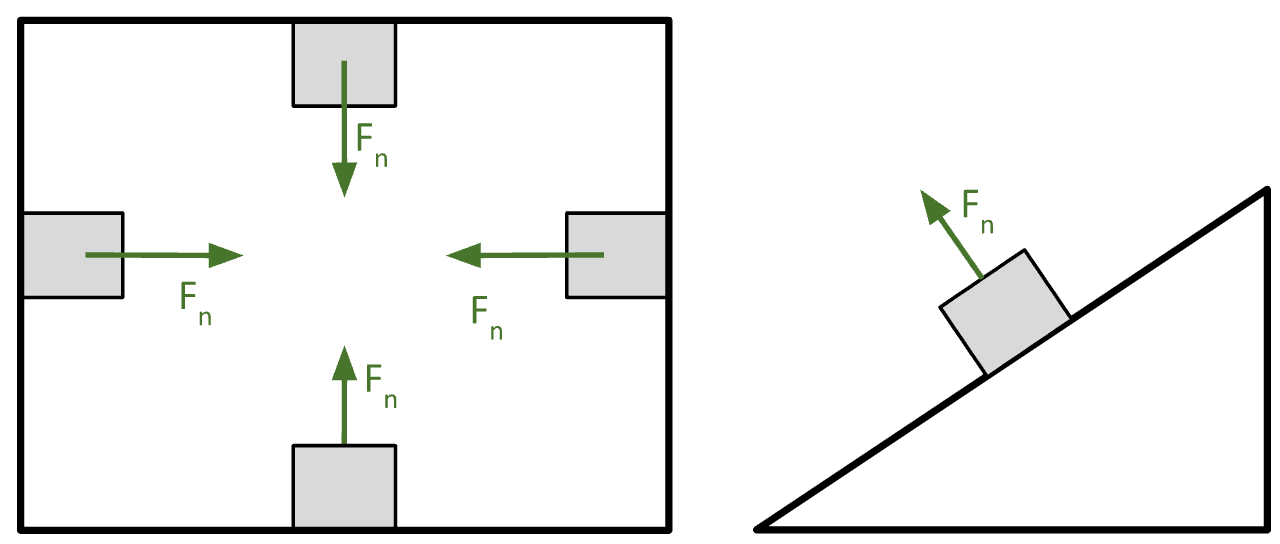
\includegraphics[width=.8\textwidth]{assets/77585bbc.png}
    \end{figure}
\end{frame}

\begin{frame}{阻力 (f) Opposing force (f)}
    \begin{itemize}
        \item 例子:Examples:
              \begin{itemize}
                  \item 固體之間的摩擦力。\\Frictional forces between solids.
                  \item 空氣阻力。\\Air resistance.
                  \item 液體阻力。\\Fluid resistance.
                  \item 刹制力。\\Braking force.
              \end{itemize}
    \end{itemize}
    \begin{figure}[h!]
        \centering
        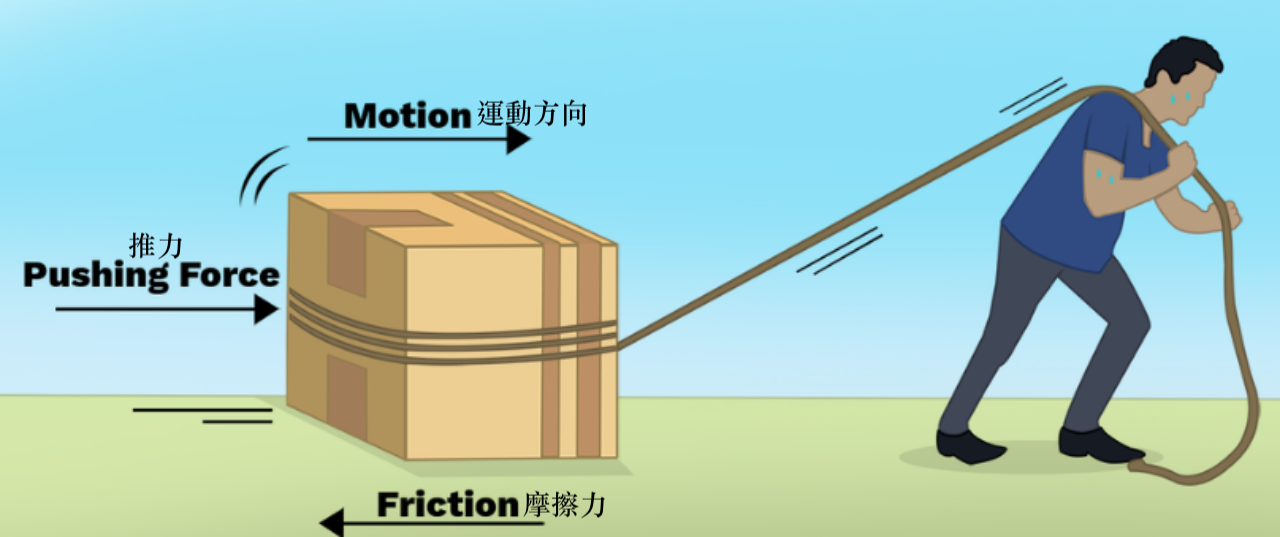
\includegraphics[width=.5\textwidth]{assets/48a9a34c.png}
    \end{figure}
\end{frame}
\begin{frame}{阻力 Opposing force}
    \begin{itemize}
        \item 防止兩個接觸面發生相對運動所產生的力。\\The force that prevents relative motion between two contacting surfaces is called frictional force.
        \item 存在一個最大量值。\\There exists a maximum magnitude.
              \begin{itemize}
                  \item 阻力隨相對運動程度的增加而增加。沒有相對運動就沒有阻力。\\Opposing force increases with the degree of relative motion. Without relative motion, there is no resistance.
                  \item 當阻力超過最大值時,阻力不會再增加。\\When the resistance exceeds the maximum value, the resistance will not increase further.
              \end{itemize}
    \end{itemize}
\end{frame}

% \begin{frame}{降低摩擦力的方法}
% \begin{columns}
%     \column{.5\textwidth}
%     水平接觸面加上塑膠小珠\\add plastic bearings
% 接觸面加上油層\\add lubricating oil between contact surfaces
% 利用氣墊導航產生氣墊\\
%     \column{.5\textwidth}

% \end{columns}


% \end{frame}
% \begin{frame}{降低流線阻力的方法}
% 流線形設計\\streamline design
% \begin{columns}
%     \column{.5\textwidth}
%     \begin{figure}[h!]
% 	\centering
% 	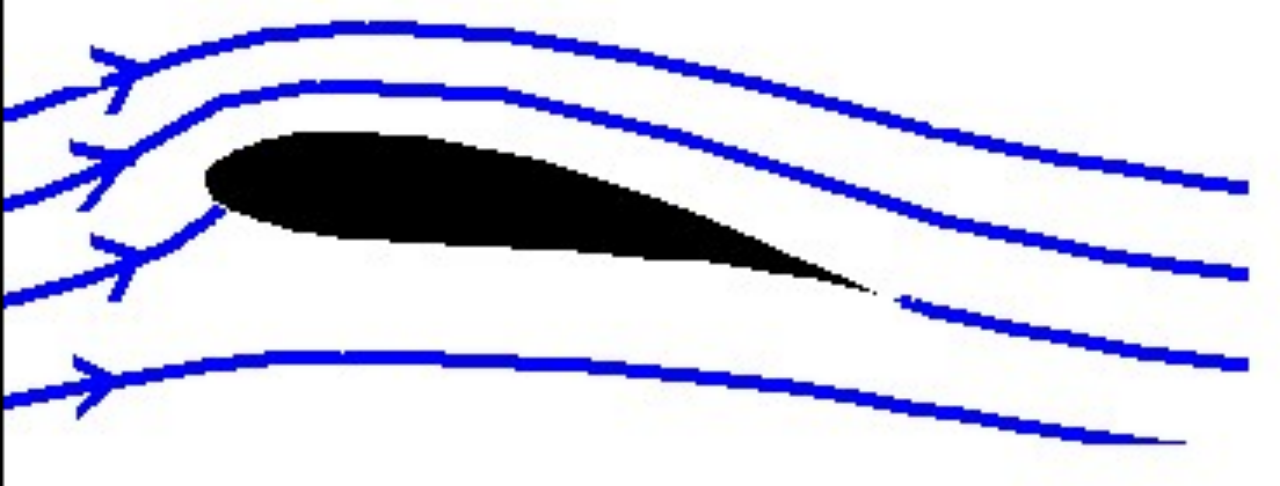
\includegraphics[width=.8\textwidth]{assets/710f9991.png}
% 	\end{figure}
%     \column{.5\textwidth}
%     \begin{figure}[h!]
% 	\centering
% 	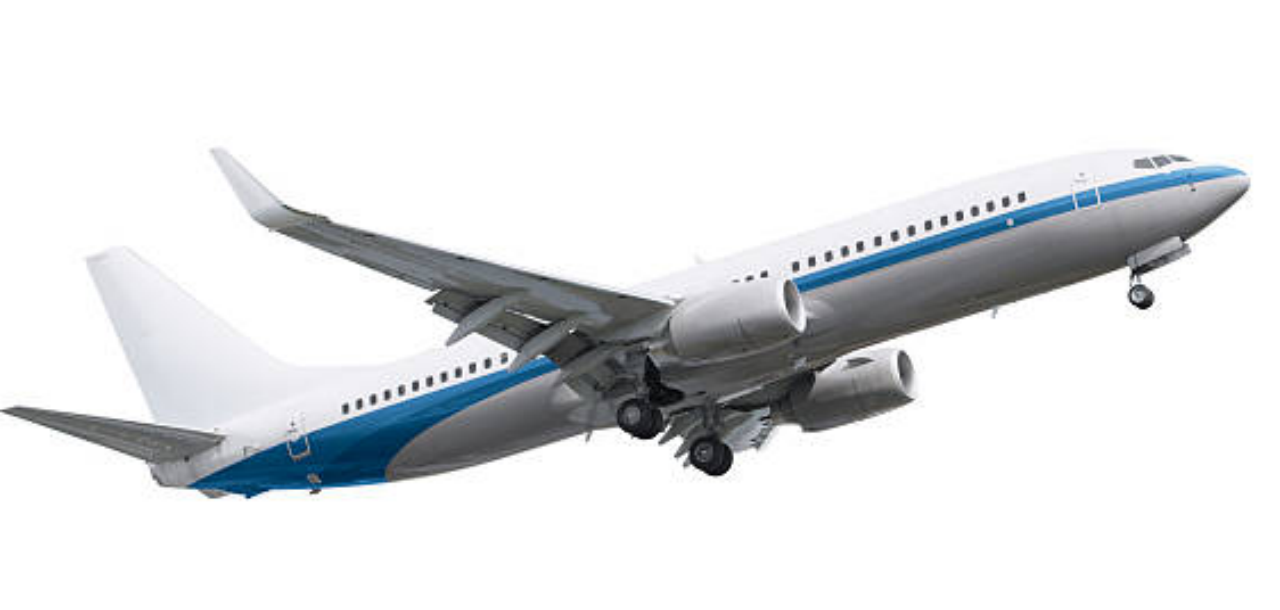
\includegraphics[width=.8\textwidth]{assets/4f685eca.png}
% 	\end{figure}
% \end{columns}
% \end{frame}

\begin{frame}{自由體圖/隔離體圖 Free body diagram}
    \begin{itemize}
        \item 顯示所有作用於物體的力。Indicates all forces acting on a body.\bigskip
    \end{itemize}
    \begin{figure}[h!]
        \centering
        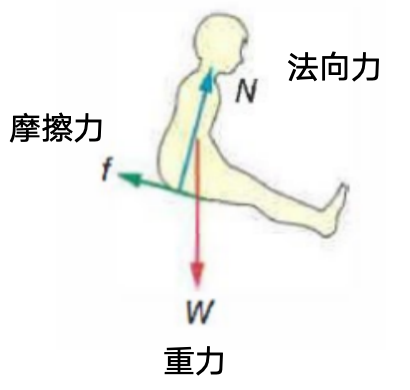
\includegraphics[width=0.5\textwidth]{assets/d2f67986.png}
    \end{figure}
\end{frame}



\begin{frame}{淨力/合力Net force/Resultant force}
    \begin{itemize}
        \item 施加於物體的所有力的向量和。\\Vector sum of all forces of an object.
    \end{itemize}\bigskip
    \begin{figure}[h!]
        \centering
        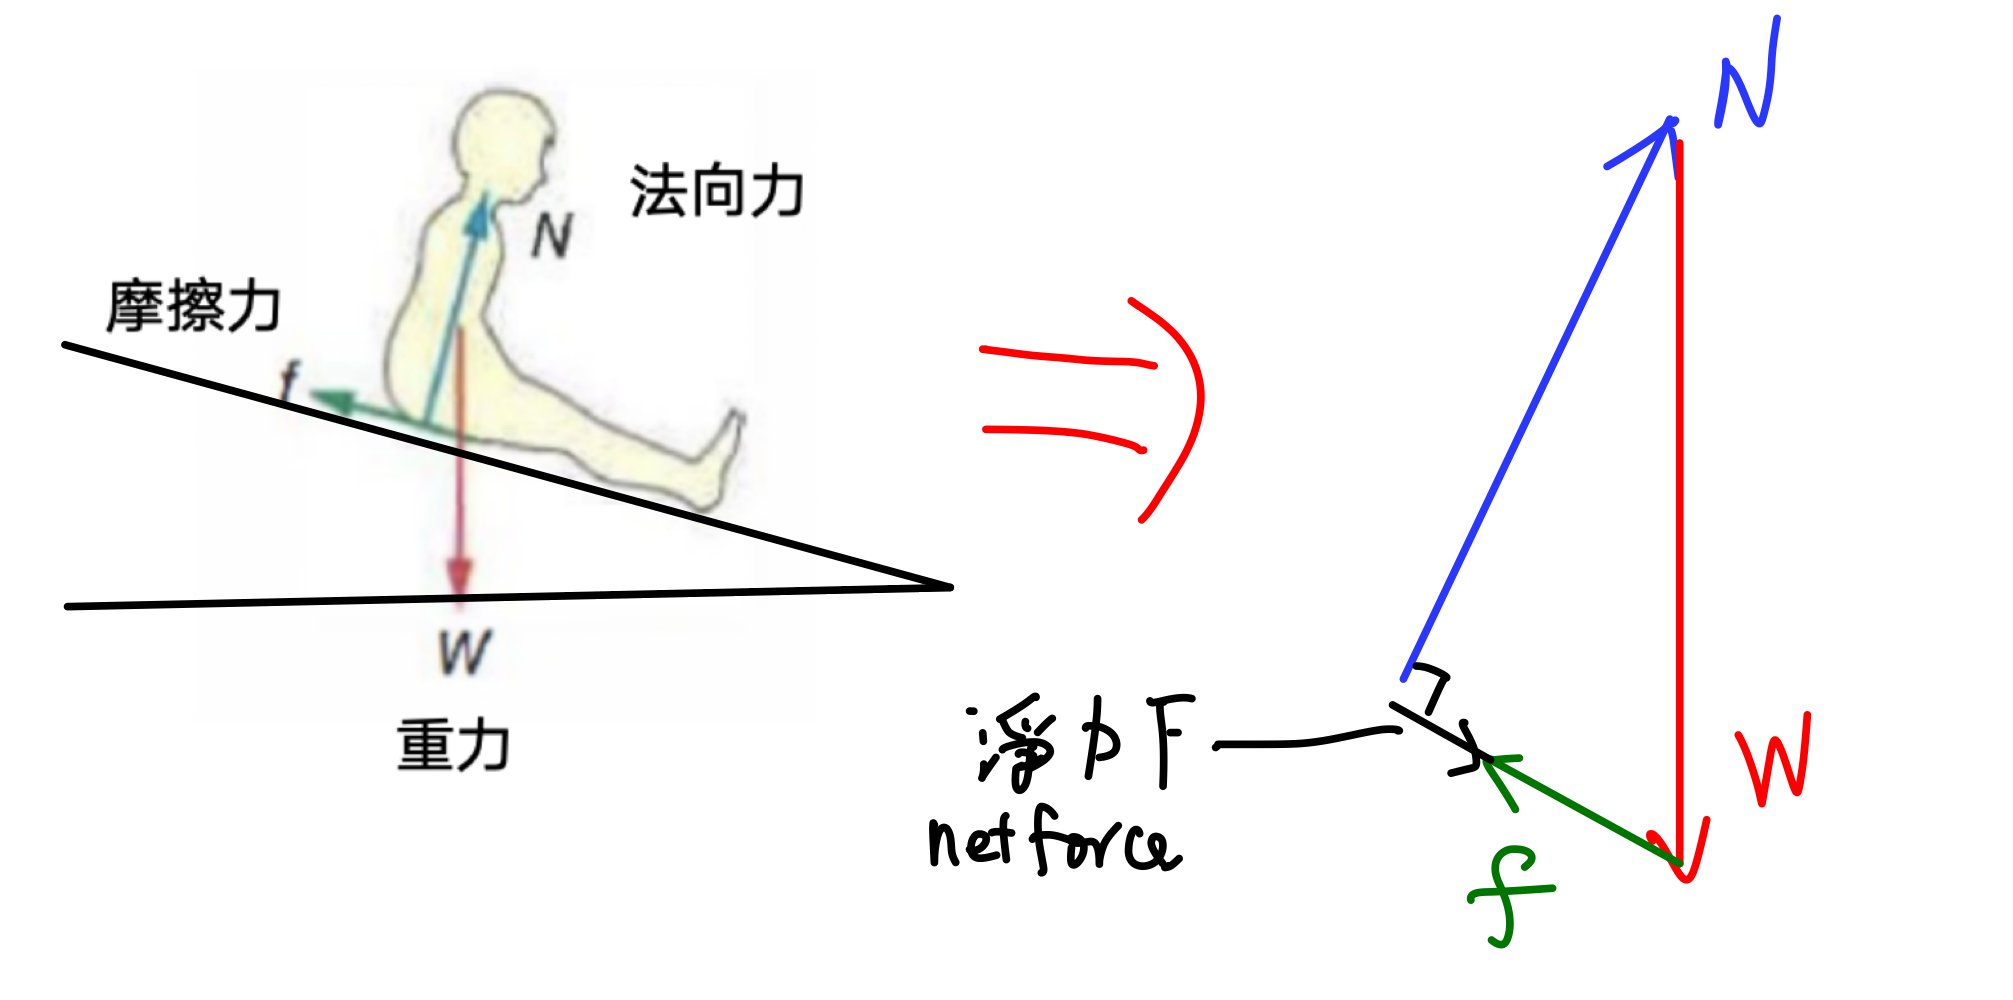
\includegraphics[width=.8\textwidth]{assets/96369bc9.png}
    \end{figure}
\end{frame}
\begin{frame}{淨力/合力Net force/Resultant force}
    \begin{figure}[h!]
        \centering
        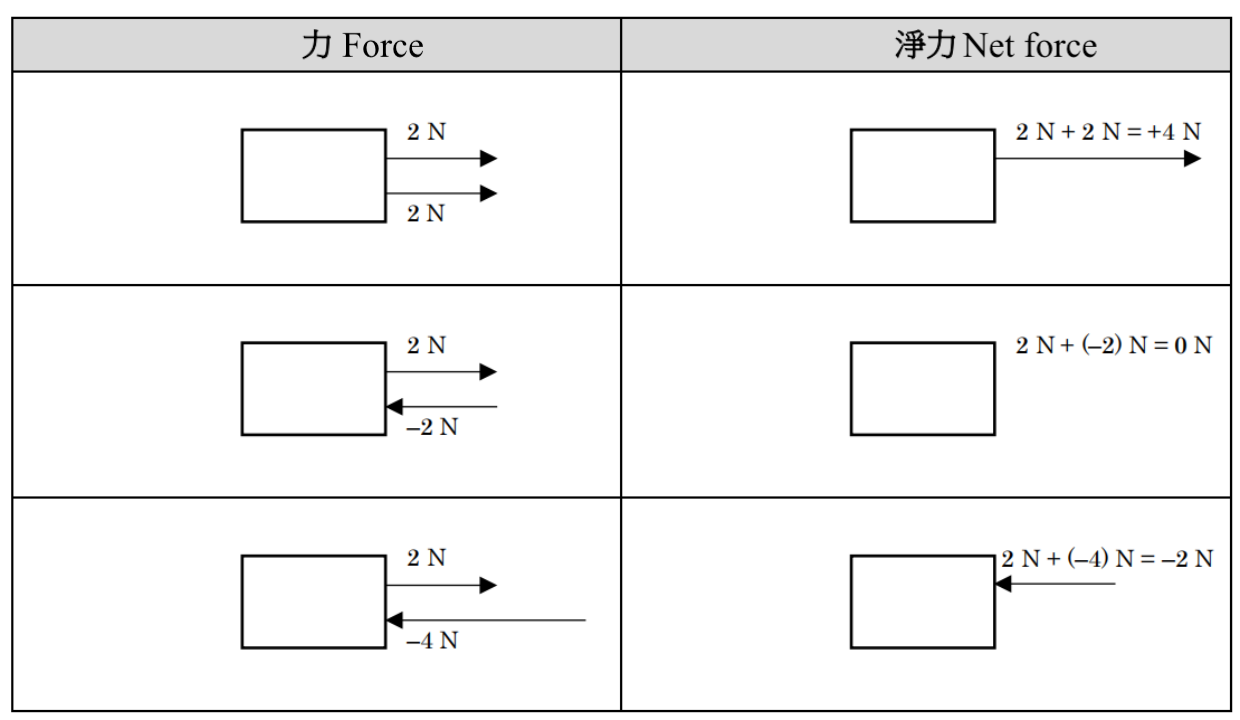
\includegraphics[width=\textwidth]{assets/5ffd7887.png}
    \end{figure}
\end{frame}
\begin{frame}{淨力/合力Net force/Resultant force}
    \begin{figure}[h!]
        \centering
        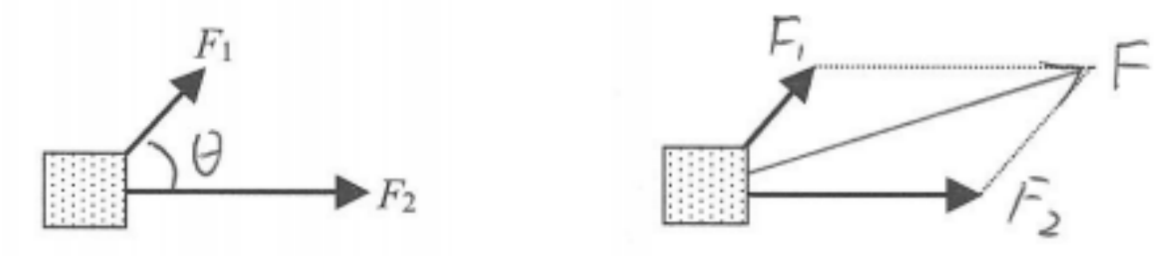
\includegraphics[width=.8\textwidth]{assets/61448695.png}
    \end{figure}
\end{frame}

\begin{frame}{力的拆解方法Force breaking into components}
    \begin{figure}[h!]
        \centering
        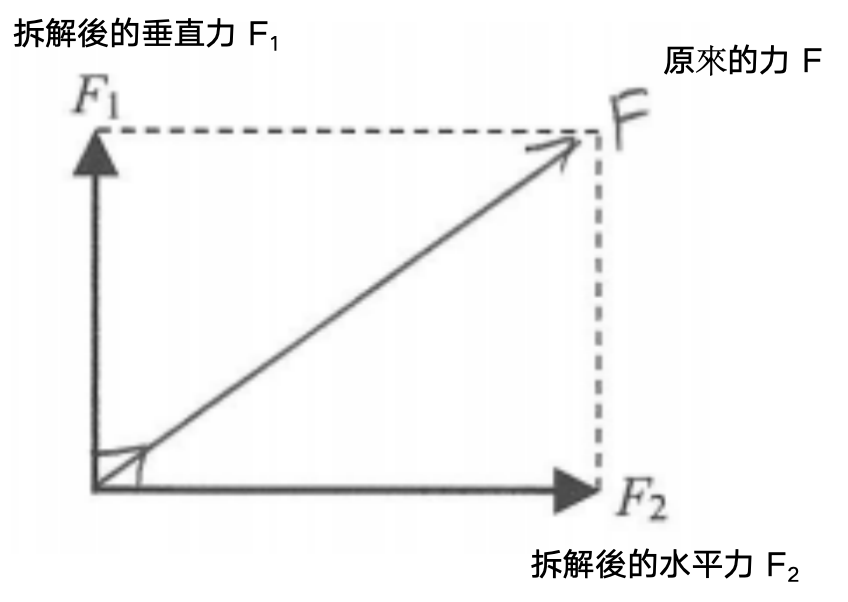
\includegraphics[width=0.66\textwidth]{assets/8695f254.png}
    \end{figure}
\end{frame}

\begin{eg}
    \begin{figure}[h!]
        \centering
        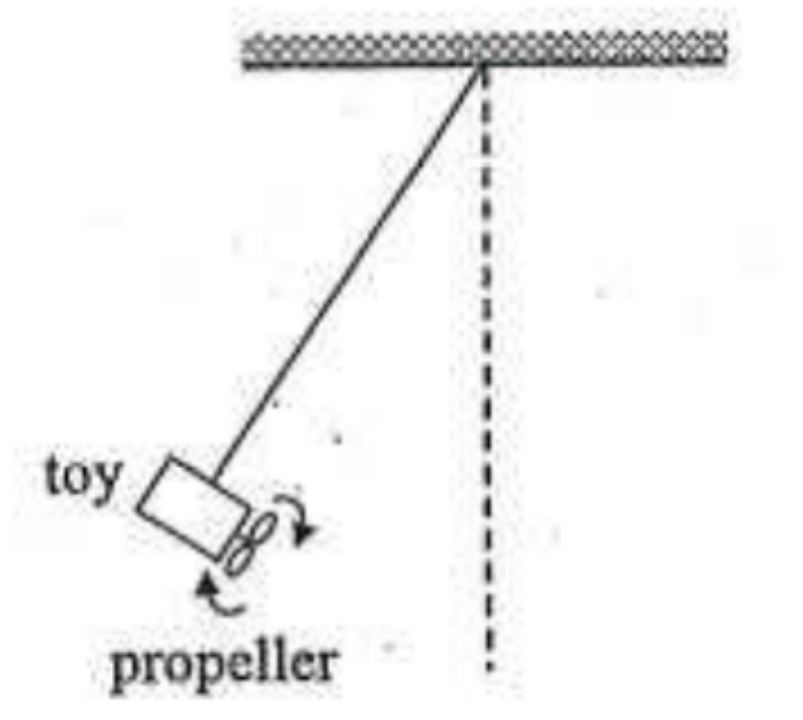
\includegraphics[width=0.35\textwidth]{assets/d7d1a80b.png}
    \end{figure}\bigskip\bigskip
    這個玩具裝了一個推進器和現在在靜止狀態。畫出這個玩具的自由體圖。\\This toy is equipped with a propeller and is currently at rest. Draw the free-body diagram of this toy.
\end{eg}

\begin{frame}[t]{例題Example}
    如圖所示,兩個量使固定的力F$_1$及F$_2$作用於同一點,當F$_1$與F$_2$的夾角$\theta$由 \dg{0} 增加至 \dg{180},求合力的量值的變化。\\(a)增加(b)減少(c)先增加後減少(d)先減少後增加\\As shown in the diagram, two forces, F$_1$ and F$_2$, are applied to the same point. When the angle $\theta$ between F$_1$ and F$_2$ increases from \dg{0} to \dg{180}, what is the change of the magnitude of the resultant force? (a) increases (b) decreases (c) increases then decreases (d) decreases then increases.
    \begin{figure}[h!]
        \centering
        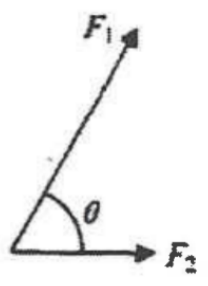
\includegraphics[width=.22\textwidth]{assets/11bd149b.png}
    \end{figure}
\end{frame}

\begin{frame}{有關力的定理Force-related laws}
    \begin{columns}
        \column{.4\textwidth}
        \begin{center}
            {\LARGE\textbf{牛頓力學定律\\\vspace{1cm}Newton's Three Laws of motion}}
        \end{center}

        \column{.4\textwidth}
        \begin{figure}[h!]
            \centering
            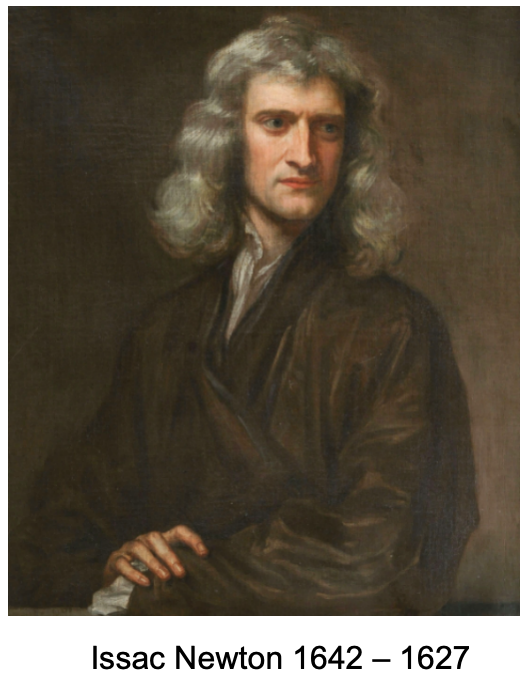
\includegraphics[width=.75\textwidth]{assets/57b990b1.png}
        \end{figure}

    \end{columns}
\end{frame}

\begin{frame}{牛頓第一定律和慣性 Newton's first law and inertia}
    \begin{alertblock}
        {牛頓第一定律 Newton's first law}
        除非受到淨力作用,否則所有物體都會保持靜止狀態或勻速直線運動狀態。 \\Unless there is a net force, the object stays at rest or moves uniformly.
    \end{alertblock}
    \begin{exampleblock}
        {慣性inertia}
        慣性是物體保持靜止或以均勻速度運動的趨勢。\\Inertia is the tendency of a body to remain at rest or moving with uniform velocity.
    \end{exampleblock}
\end{frame}
\begin{frame}{牛頓第一定律和慣性 Newton's first law and inertia}
    \begin{itemize}
        \item 慣性使物體繼續以勻速移動。\\Objects keeps its uniform speed because of inertia.\bigskip\bigskip
    \end{itemize}
    \begin{columns}
        \column{.33\textwidth}
        \begin{figure}[h!]
            \centering
            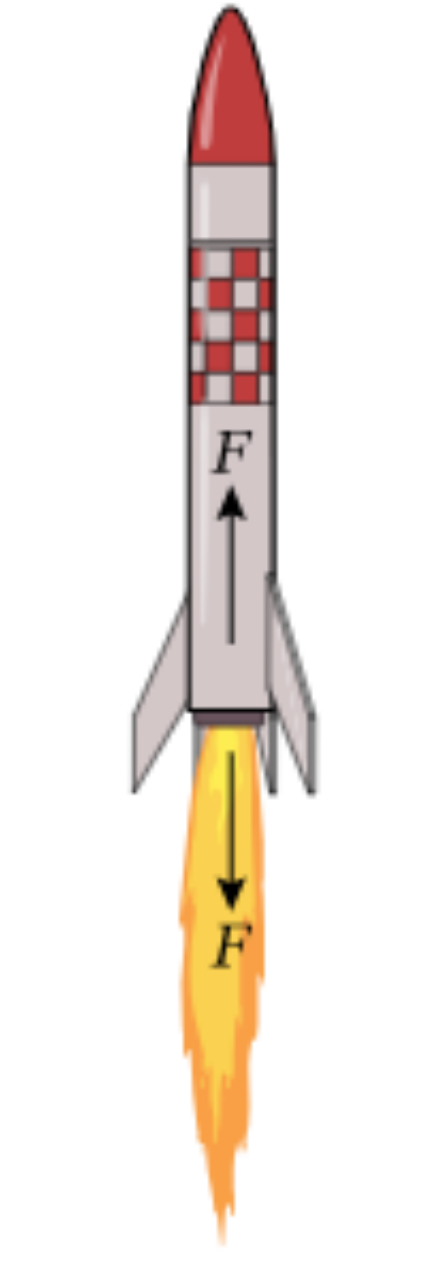
\includegraphics[width=0.4\textwidth]{assets/c32f5f7b.png}
        \end{figure}
        \column{.33\textwidth}
        \begin{figure}[h!]
            \centering
            
\includegraphics[width=.85\textwidth]{assets/b65bc2e1.png}
        \end{figure}
        \column{.33\textwidth}
        \begin{figure}[h!]
            \centering
            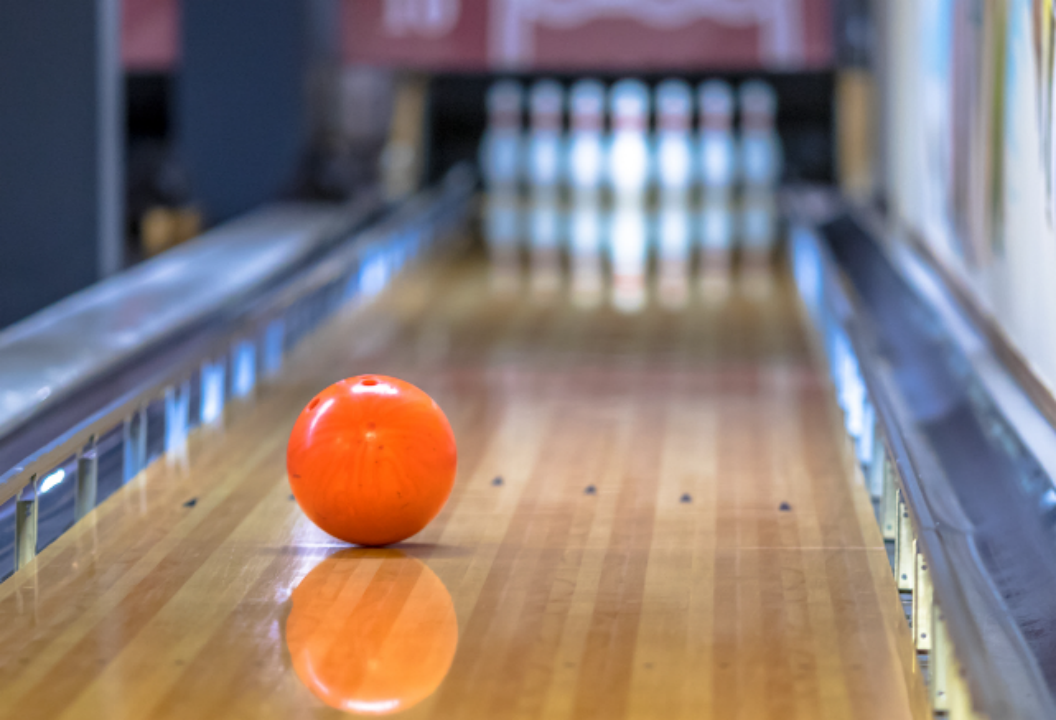
\includegraphics[width=.85\textwidth]{assets/888883a6.png}
        \end{figure}
    \end{columns}

\end{frame}

\begin{frame}{安全帶的應用Application of seat belts}
    \begin{itemize}
        \item 當移動中的車子突然停車,因為慣性乘客會繼續前進。\\When a moving vehicle suddenly stops, due to inertia, passengers will continue to move forward.
        \item 安全帶可以防止乘客被拋出車外。\\Seat belts are designed to prevent passengers from being thrown out of the vehicle.
    \end{itemize}
    \begin{figure}[h!]
        \centering
        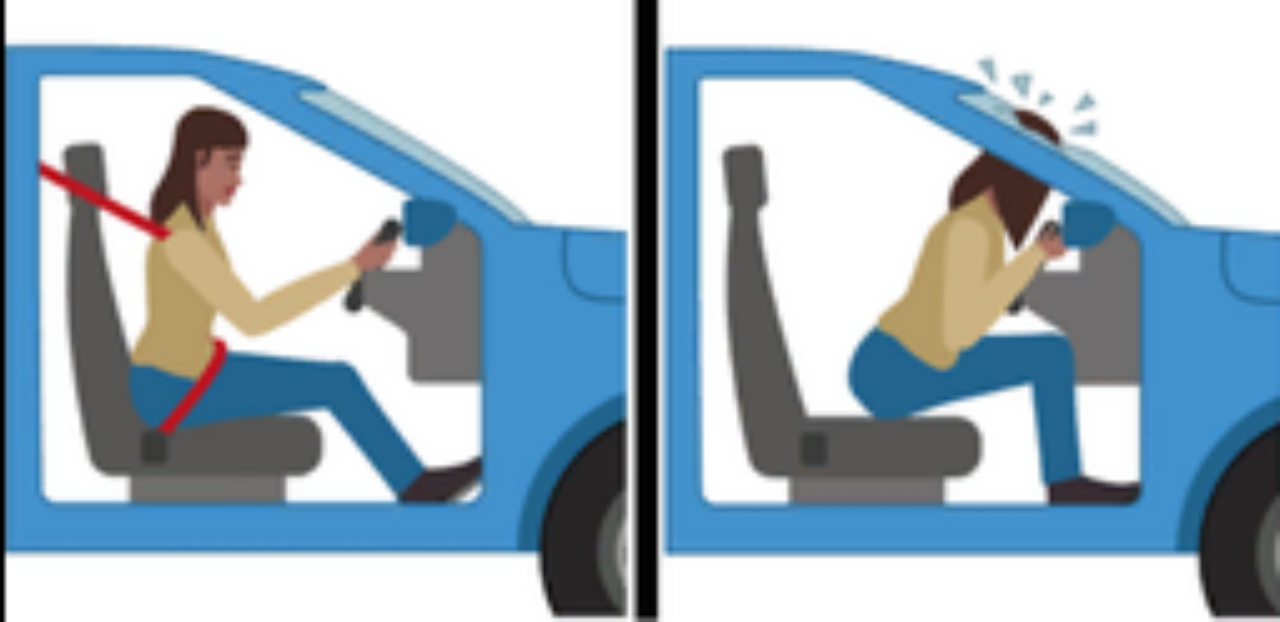
\includegraphics[width=.5\textwidth]{assets/88ea2a86.png}
    \end{figure}
\end{frame}

\begin{frame}{牛頓第一定律和慣性 Newton's first law and inertia}
    \begin{itemize}
        \item 慣性使物體繼續靜止。 \\A body will remain at rest due to its inertia
    \end{itemize}
    \begin{figure}[h!]
        \centering
        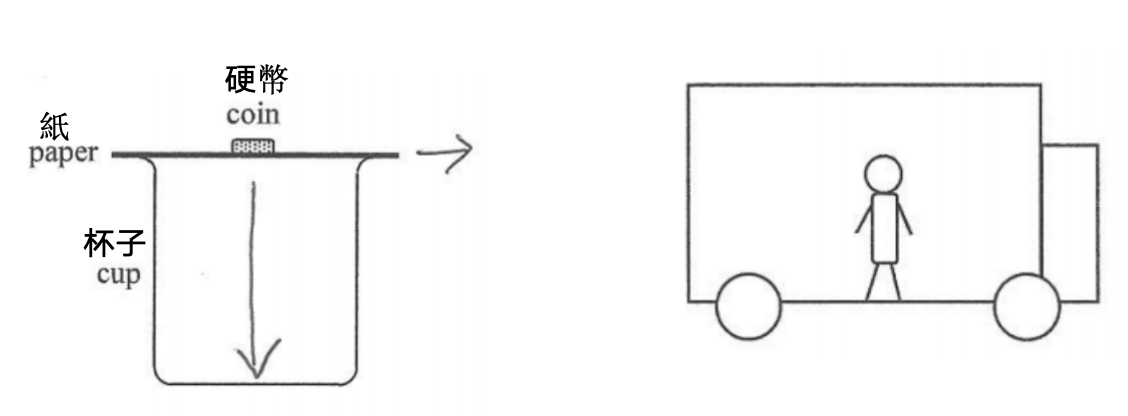
\includegraphics[width=0.85\textwidth]{assets/d5349655.png}
    \end{figure}
\end{frame}

\begin{frame}{牛頓第一定律和慣性 Newton's first law and inertia}
    \begin{itemize}
        \item 慣性使物體繼續靜止。 \\A body will remain at rest due to its inertia.
    \end{itemize}
    \begin{columns}
        \column{.6\textwidth}
        \begin{itemize}
            \item 慢拉線$\Rightarrow$上面先斷\\string is pulled slowly $\Rightarrow$ upper string breaks.
                  \begin{itemize}
                      \item 上面部分承受更大的張力。\\upper string breaks because it has greater tension.
                  \end{itemize}
            \item 快拉線 $\Rightarrow$ 下面先斷\\string is pulled quickly $\Rightarrow$ lower string breaks.
                  \begin{itemize}
                      \item 物件傾向保持靜止狀態。\\because the block tends to remain at rest.
                  \end{itemize}
        \end{itemize}
        \column{.4\textwidth}
        \begin{figure}[h!]
            \centering
            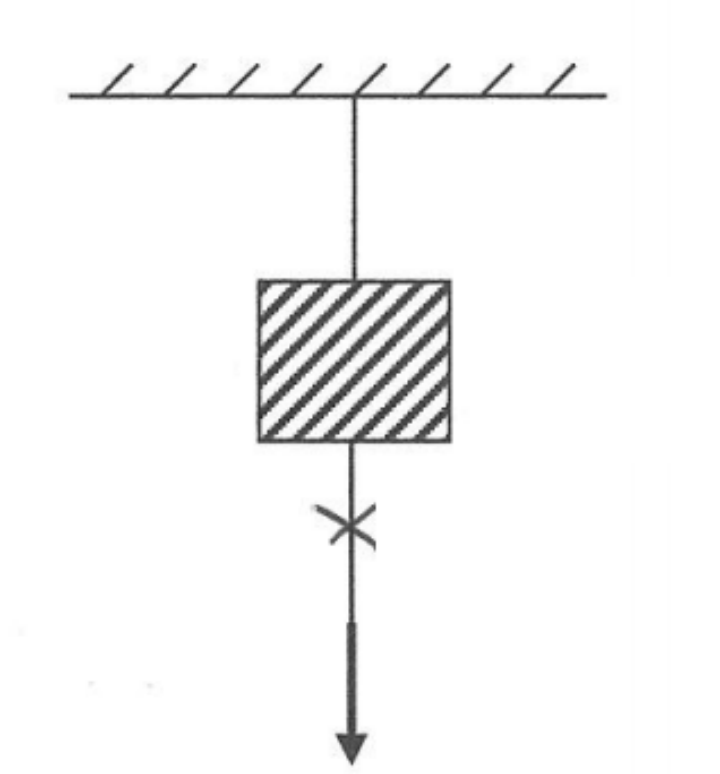
\includegraphics[width=.8\textwidth]{assets/842a74ec.png}
        \end{figure}
    \end{columns}
\end{frame}



\begin{frame}{牛頓第二定律 Newton's second law}
    \begin{alertblock}
        {牛頓第二定律 Newton's second law}
        \begin{equation}
            \vec{F}=m\vec{a}
        \end{equation}
    \end{alertblock}
    \begin{itemize}

        \item 物件受到的淨力 F 與物件的質量 m 及加速度 a 成正比,且淨力和加速度方向相同,且量值滿足 $F=m a$ 。 \\An object of mass m accelerates at a when it is experiencing a net force F, then the directions of F and a are the same, and their magnitudes fulfil $F=m a$ .
        \item 淨力、質量和加速度分別採用S.I.單位牛頓(N)、千克(kg)和米每平方秒(\acc{})。 \\the net force, mass and acceleration are in the S.I. units, Newton (N), kilograms (kg) and meters per second squared (\acc{}) respectively.
    \end{itemize}
\end{frame}

\begin{eg}
    一塊起始靜止的方塊放在光滑的桌子上,被一個水平的恆定力 F 推動。利用牛頓運動定律,解釋為什麼這個方塊應該開始移動。\\A block which is initially at rest and placed on a smooth table is being pushed by a horizontal constant force F. Using Newton's Law of Motion, explain why the block should start to move.
    \begin{itemize}
        \item [解] 施加在方塊上垂直方向的合力(重力和法向反作用力)是平衡的。水平方向有非零的淨力F作用於方塊上。\\根據牛頓第二定律,方塊應該會有與力同方向的加速度。
        \item [Ans] The vertical forces (weight and normal reaction) are balanced, While there is an unbalanced horizontal resultant force F acting on the block.\\By Newton's 2nd law, the block should have acceleration with same direction to the force.
    \end{itemize}
\end{eg}

\begin{eg}
    一個球質量為 4 kg,它被輕推了一下後,以速率\vel{2}運動。10 s後,它停了下來。 \\The mass of a ball is 4 kg, after being pushed, it moves at \vel{2}. After moving for 10 s, it stops.
    \begin{itemize}
        \item[(a)] 求球與地面間的摩擦力。 \\Find the friction between the ball and the ground.
    \end{itemize}
\end{eg}
\begin{eg}
    一個球質量為 4 kg,它被輕推了一下後,以速率\vel{2}運動。10 s後,它停了下來。 \\The mass of a ball is 4 kg, after being pushed, it moves at \vel{2}. After moving for 10 s, it stops.
    \begin{itemize}
        \item[(b)] 如果摩擦力減半而其他因素不變,球移動的距離是多少? \\If the friction reduces by half and the other factors stay unchanged, what is the distance covered by the ball?
    \end{itemize}
\end{eg}
\begin{eg}
    一個球質量為 4 kg,它被輕推了一下後,以速率\vel{2}運動。10 s後,它停了下來。 \\The mass of a ball is 4 kg, after being pushed, it moves at \vel{2}. After moving for 10 s, it stops.
    \begin{itemize}
        \item[(c)] 如果摩擦力加倍而其他因素不變,球移動的時間是? \\If the friction doubles and other factors stay unchanged, what is the moving time of the ball?
    \end{itemize}
\end{eg}


\begin{eg}
    一個男孩的質量是 30 kg。他以\vel{5}垂直到達水面且他最深下降至 \qty{2}{m}。求水對男孩施力的量值。\\ The mass of a boy is 30 kg. He reaches the water surface at \vel{5} vertically downward and he reaches \qty{2}{m} of depth at most. Find the magnitude of the force acted on the boy by water.
\end{eg}

\begin{frame}{拆力相關題目Problems about breaking forces}
    \begin{itemize}
        \item 把力分解成水平和垂直方向。\\Breaking down the force into vertical and horizontal components.
              \begin{itemize}
                  \item 然後把該方向的所有力放一邊,ma放另一邊。\\Then, all the forces in that direction are placed on one side, while ma (mass times acceleration) is placed on the other side.
                  \item 如果是靜止/勻速,一邊方向的所有力=另一邊方向的所有力。\\If the object is at rest or moving at a constant velocity, the sum of all forces in one direction is equal to the sum of all forces in the opposite direction.
              \end{itemize}
        \item 斜坡問題:Problems related to a slope:
              \begin{itemize}
                  \item 把力分解成沿鈄坡,和垂直於斜坡。\\Breaking down the force into direction along the plane and perpendicular to the plane.
              \end{itemize}
    \end{itemize}
\end{frame}

\begin{frame}[t]{例題Example}
    \begin{figure}[h!]
        \centering
        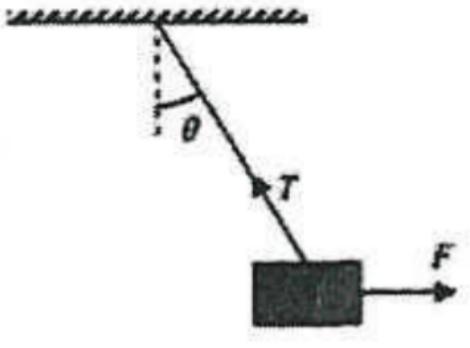
\includegraphics[width=0.3\textwidth]{assets/0b66fd6a.png}
    \end{figure}
    % 上圖中,一方塊以一繩子掛於天花板,水平力F作用在該方塊上。於平衡狀態時,繩子和豎直成角$\theta$,而繩子的張力為T。以F和$\theta$表示該方塊的重量。\\In the given diagram, a block is suspended from the ceiling by a rope, and a horizontal force F is applied to the block. In the equilibrium state, the rope forms an angle $\theta$ with the vertical, and the tension in the rope is T. Find the weight of the block in terms of F and $\theta$. 
    以F和$\theta$表示方塊的重量。\\Find the weight of the block in terms of F and $\theta$.
\end{frame}

\begin{eg}
    揚浩將手推車推上斜坡。他施於手推車的力平行於斜坡,量值為 200 N。斜坡與水平線的夾角為 \oc{10}。手推車連貨物的質量為 50 kg,斜坡施於手推車的摩擦力為 80 N。\\Y.H. pushes a trolley up along a slope. The force that he acts on the trolley is parallel to the slope, and the magnitude is 200 N. The inclination of the slope is \oc{10}. The total mass of the trolley and the goods inside is 50 kg, the friction between the slop and the trolley is 80 N.

    \begin{itemize}
        \item[(a)] 斜坡施於手推車的法向力,量值是多少?\\What is the magnitude of the normal force acting on the trolley by the slope?
    \end{itemize}

\end{eg}
\begin{eg}
    揚浩將手推車推上斜坡。他施於手推車的力平行於斜坡,量值為 200 N。斜坡與水平線的夾角為 \dg{10}。手推車連貨物的質量為 50 kg,斜坡施於手推車的摩擦力為 \qty{80}{N}。\\Y.H. pushes a trolley up along a slope. The force that he acts on the trolley is parallel to the slope, and the magnitude is 200 N. The inclination of the slope is \dg{10}. The total mass of the trolley and the goods inside is 50 kg, the friction between the slop and the trolley is \qty{80}{N}.

    \begin{itemize}
        \item[(b)] 求手推車的加速度量值。\\Calculate the magnitude of the acceleration of the trolley.
    \end{itemize}
\end{eg}

\begin{frame}{滑輪問題Pulley problems}
    \begin{itemize}
        \item \textbf{輕質不可延伸}的繩子:繩子上每一個點的張力皆為\textbf{零}。\\A \textbf{light} and \textbf{inextensible} string: The tension at every point on the string is \textbf{zero}.
        \item \textbf{光滑}滑輪:滑輪兩邊的張力量值\textbf{相等}。\\\textbf{Smooth} pulley: magnitudes of tension on both sides of pulley are equal.
    \end{itemize}
    \begin{figure}[h!]
        \centering
        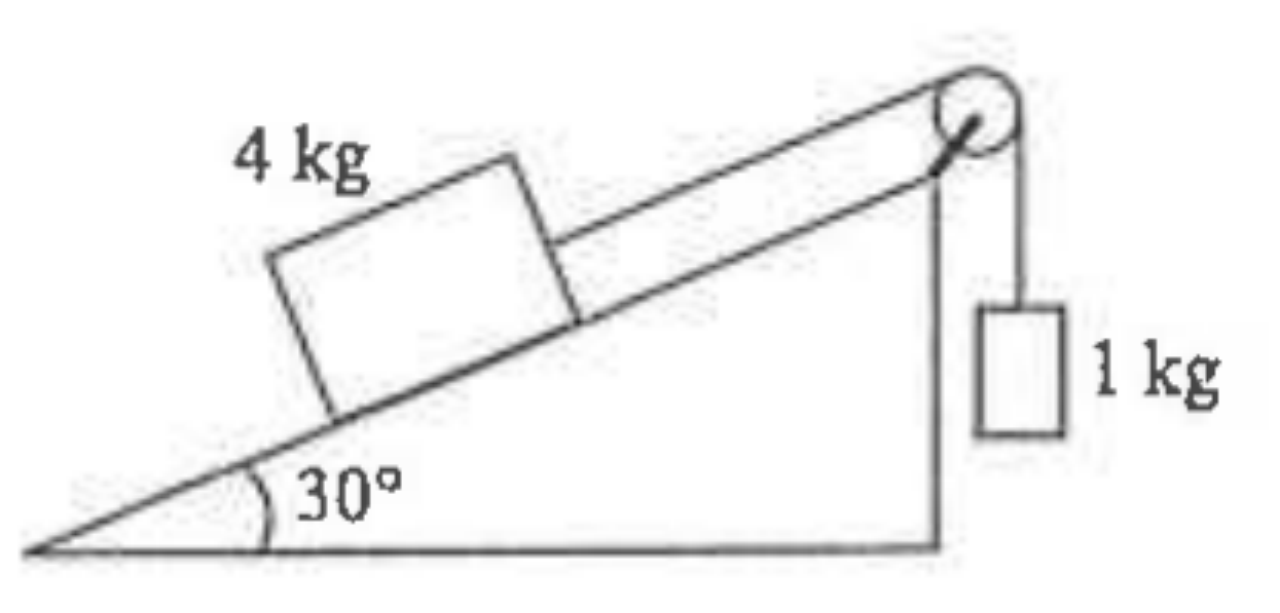
\includegraphics[width=0.4\textwidth]{assets/54dc796f.png}
    \end{figure}
\end{frame}


\begin{eg}
    \begin{figure}[h!]
        \centering
        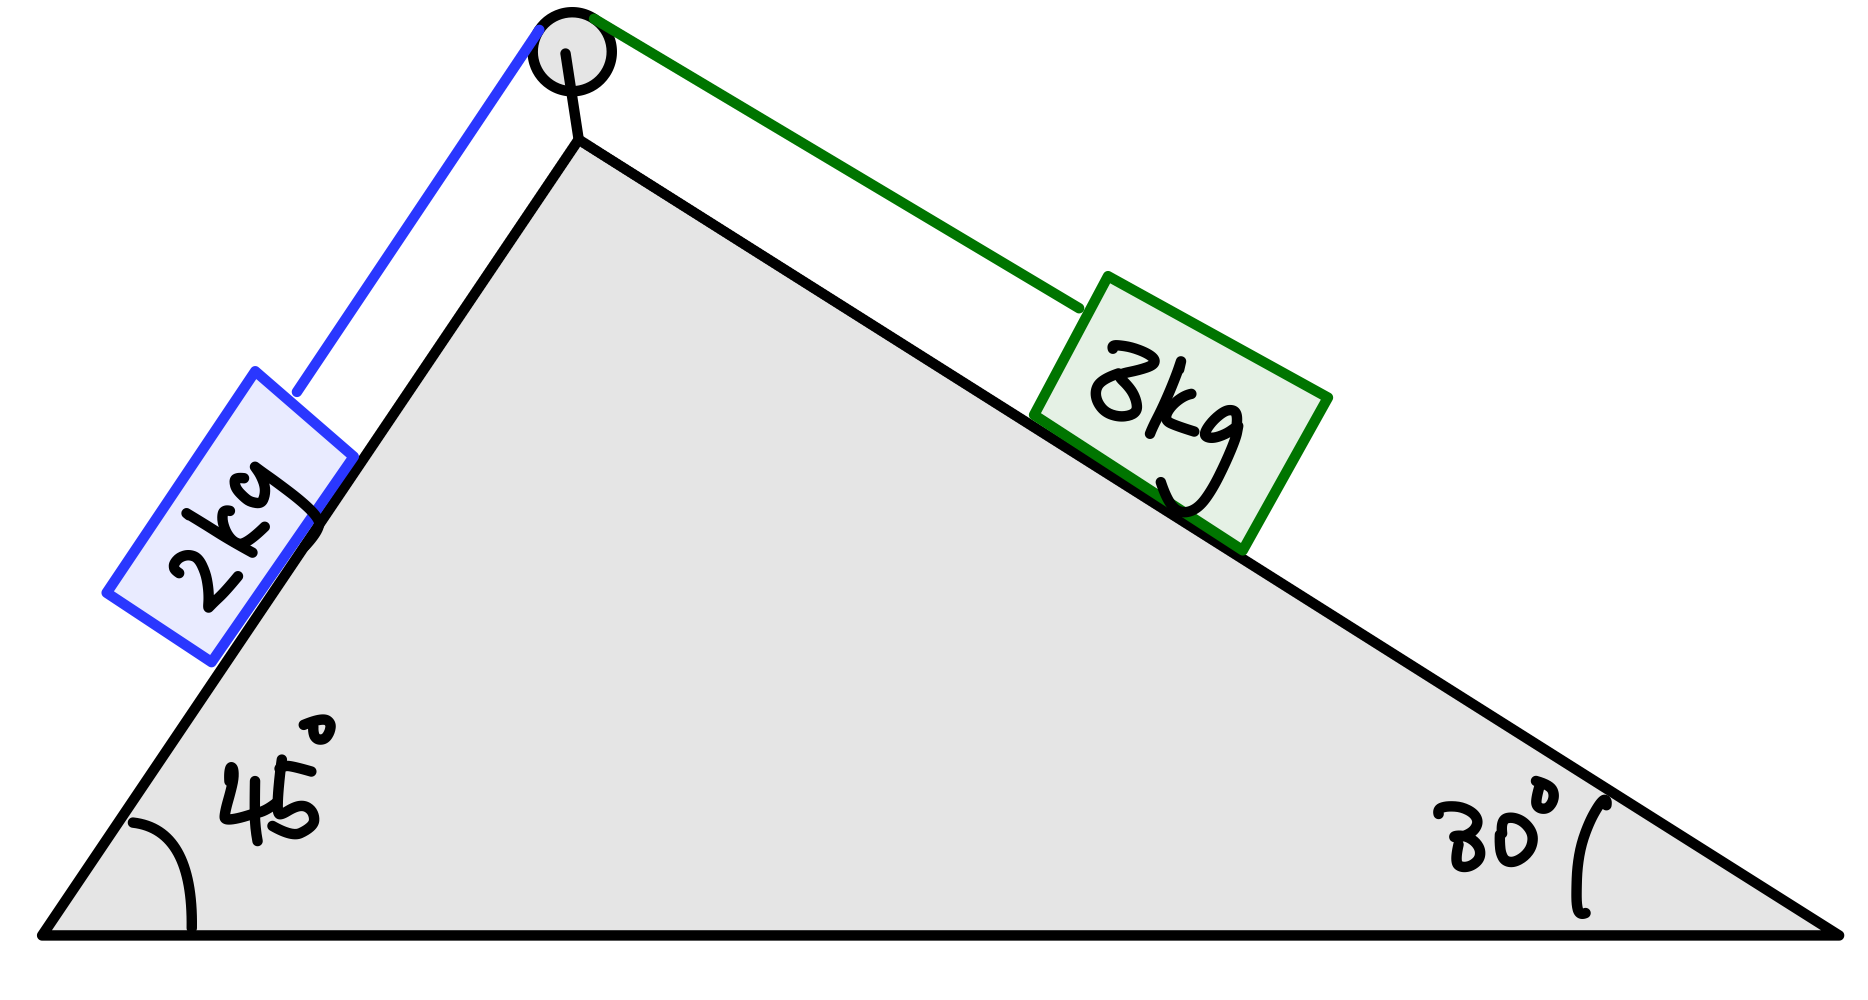
\includegraphics[width=0.4\textwidth]{assets/a078f185.png}
    \end{figure}
    所有表面光滑,取重力加速度 g = \acc{9.81}。求繩子的張力。\\All surfaces are smooth, and the gravitational acceleration is given by g = \acc{9.81}. Find the tension in the string.
\end{eg}



\begin{eg}
    \begin{figure}[h!]
        \centering
        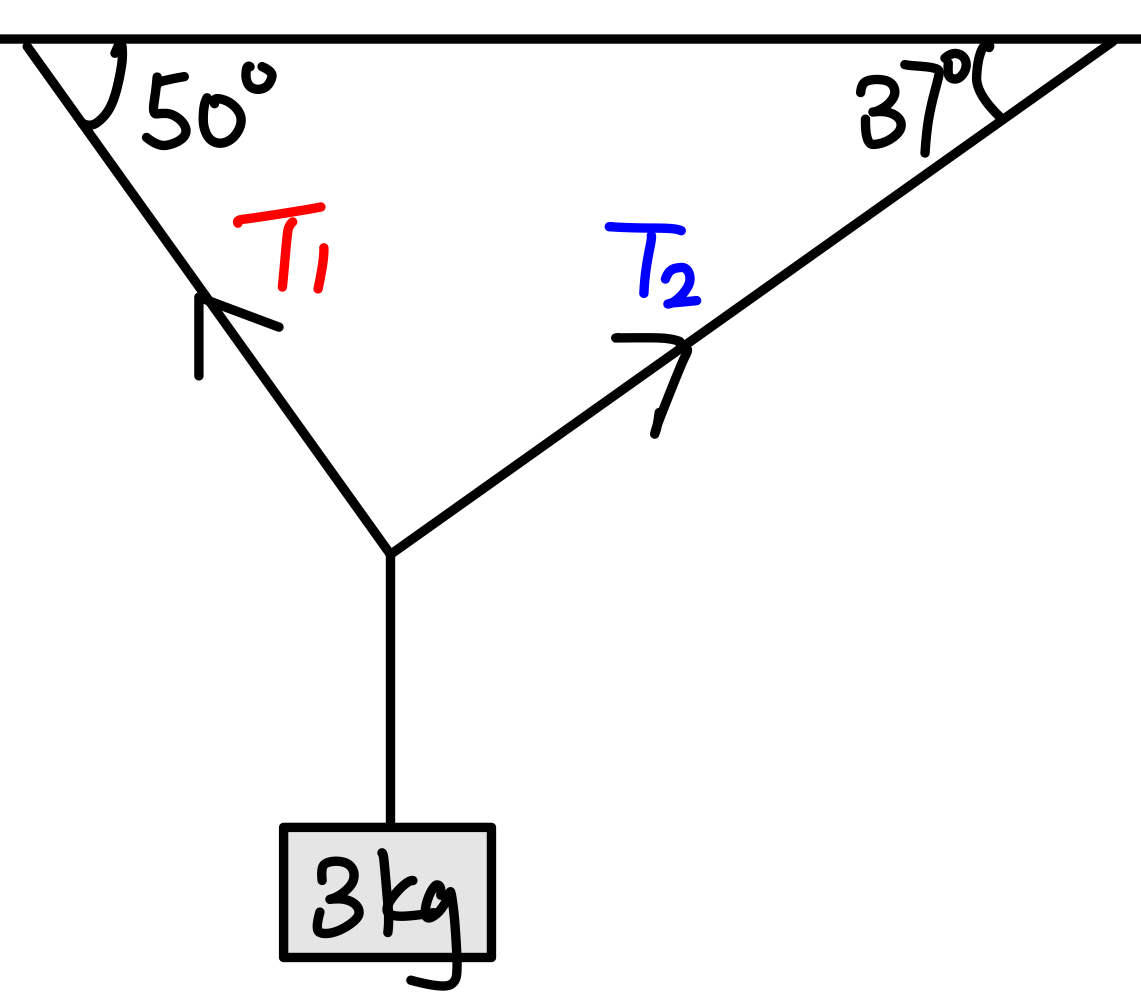
\includegraphics[width=.3\textwidth]{assets/ce5681cb.png}
    \end{figure}
    取重力加速度 g = \acc{9.81}。求繩子的張力T$_1$和T$_2$。\\the acceleration due to gravity is given by g = \acc{9.81}. Find the tensions T$_1$, T$_2$ in the string.
\end{eg}

\begin{frame}{升降機問題Elevator problems}
    假設這人有50kg, 取$g$ = \acc{10}

    \begin{columns}
        \column{.65\textwidth}
        \begin{itemize}
            \setlength{\itemsep}{10pt}
            \item 電梯是均速率\\the elevator is constant velocity: $N=mg=500$N
            \item 電梯以\acc{1}向上加速\\acceleration upwards with \acc{1}: \\$\Rightarrow N-mg=ma$\\$\Rightarrow N=550$N\\感覺重了。feels heavier.

            \item 電梯以\acc{1}向下加速\\acceleration downwards with \acc{1}: \\$\Rightarrow mg-N=ma$\\$\Rightarrow N=450$N\\感覺輕了。feels lighter.
                  % \item 電梯以$>$ \acc{g} 向下加速\\the elevator accelerates downwards with $>$ \acc{g}: N=0
                  % \item N=表觀重量apparant weight
        \end{itemize}
        \column{.3\textwidth}
        \begin{figure}[h!]
            \centering
            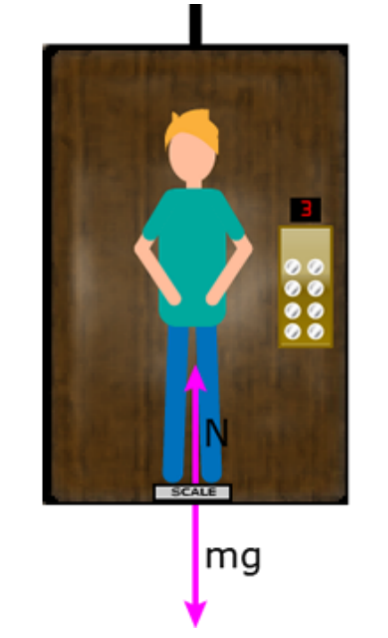
\includegraphics[width=\textwidth]{assets/6596ff5b.png}
        \end{figure}
    \end{columns}
\end{frame}
\begin{frame}{升降機問題Elevator problems}
    假設這人有50kg, 取$g$ = \acc{10}

    \begin{columns}
        \column{.65\textwidth}
        \begin{itemize}
            \setlength{\itemsep}{15pt}

            \item 電梯以 $>$ $g$\acc{} 向下加速\\acceleration downwards with $>$ $g$ \qty{}{m.s^{-2}}: \\$\Rightarrow N=0$
            \item $N=$ \textbf{表觀重量} \textbf{Apparant weight}
        \end{itemize}
        \column{.3\textwidth}
        \begin{figure}[h!]
            \centering
            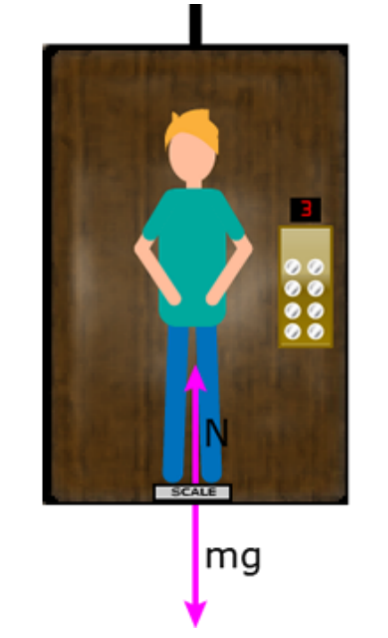
\includegraphics[width=\textwidth]{assets/6596ff5b.png}
        \end{figure}
    \end{columns}
\end{frame}

\begin{frame}{流體阻力Fluid resistance}
    \begin{exampleblock}
        {流體阻力Fluid resistance}
        \begin{equation}
            f=k \;\rho\; v^2\; A
        \end{equation}
    \end{exampleblock}
    \begin{itemize}
        \item k = 常數constant, $\rho$ = 流體密度fluid density, $v$ = 速率speed, \\$A$ = 橫截面面積cross section area
              % \item 跳傘員不開跳傘降落時,\\When skydiver falls without parachute,
              % \begin{itemize}
              %     \item 加速度向下 accelerates downwards: $W-f=ma$
              %     \item v逐漸增加gradually increases $\Rightarrow$ f 逐漸增加gradually increases
              % \end{itemize}

    \end{itemize}
    \bigskip
    \begin{figure}[h!]
        \centering
        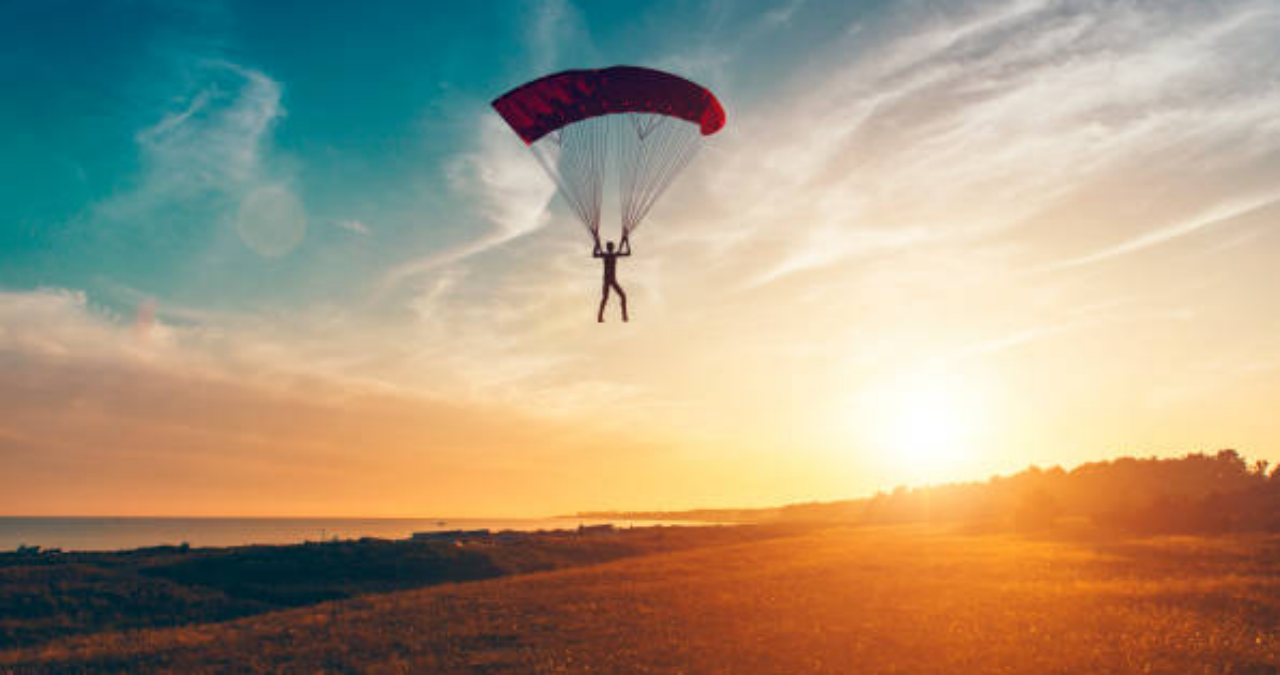
\includegraphics[width=.4\textwidth]{assets/31e14542.png}
    \end{figure}
\end{frame}
\begin{frame}{流體阻力Fluid resistance}
    \begin{itemize}
        \item 跳傘員不開跳傘降落時,\\When skydiver falls without parachute,
              \begin{itemize}
                  \item 加速度向下 accelerates downwards: $W-f=ma$
                  \item v逐漸增加gradually increases $\Rightarrow$ f 逐漸增加gradually
                  \item 直到f 完全扺消 W,淨力變成零:  $W-f=0$ \\Eventually f compensate completely W, net force is zero:  $W-f=0$
                  \item 加速度為零,以\textbf{恆定}的\textbf{終端速率}繼續落下。\\Acceleration is zero, continues falling with \textbf{constant} \textbf{terminal speed}.
              \end{itemize}
    \end{itemize}
    \begin{figure}[h!]
        \centering
        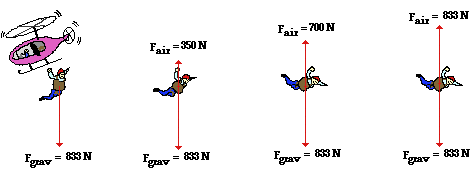
\includegraphics[width=.7\textwidth]{assets/e052106e.png}
    \end{figure}
\end{frame}
\begin{frame}{流體阻力Fluid resistance}
    \begin{itemize}
        \item 當在終端速率的跳傘員突然打開跳傘,\\When skydiver opens his parachute with terminal speed,
              \begin{itemize}
                  \item 橫截面面積突然增加,f突然增加。\\Cross section area increases suddenly, and so f increase suddenly.
                  \item 淨力向上,跳傘員向下減速。\\Net force is upwards, i.e. skydiver decelerates downwards.
                  \item f持續下降至淨力為零。\\f continuously decreases until net force becomes zero.
                  \item 以\textbf{更低}的終端速率落下。\\Falling with \textbf{lower} terminal speed.
              \end{itemize}
    \end{itemize}

    \begin{figure}[h!]
        \centering
        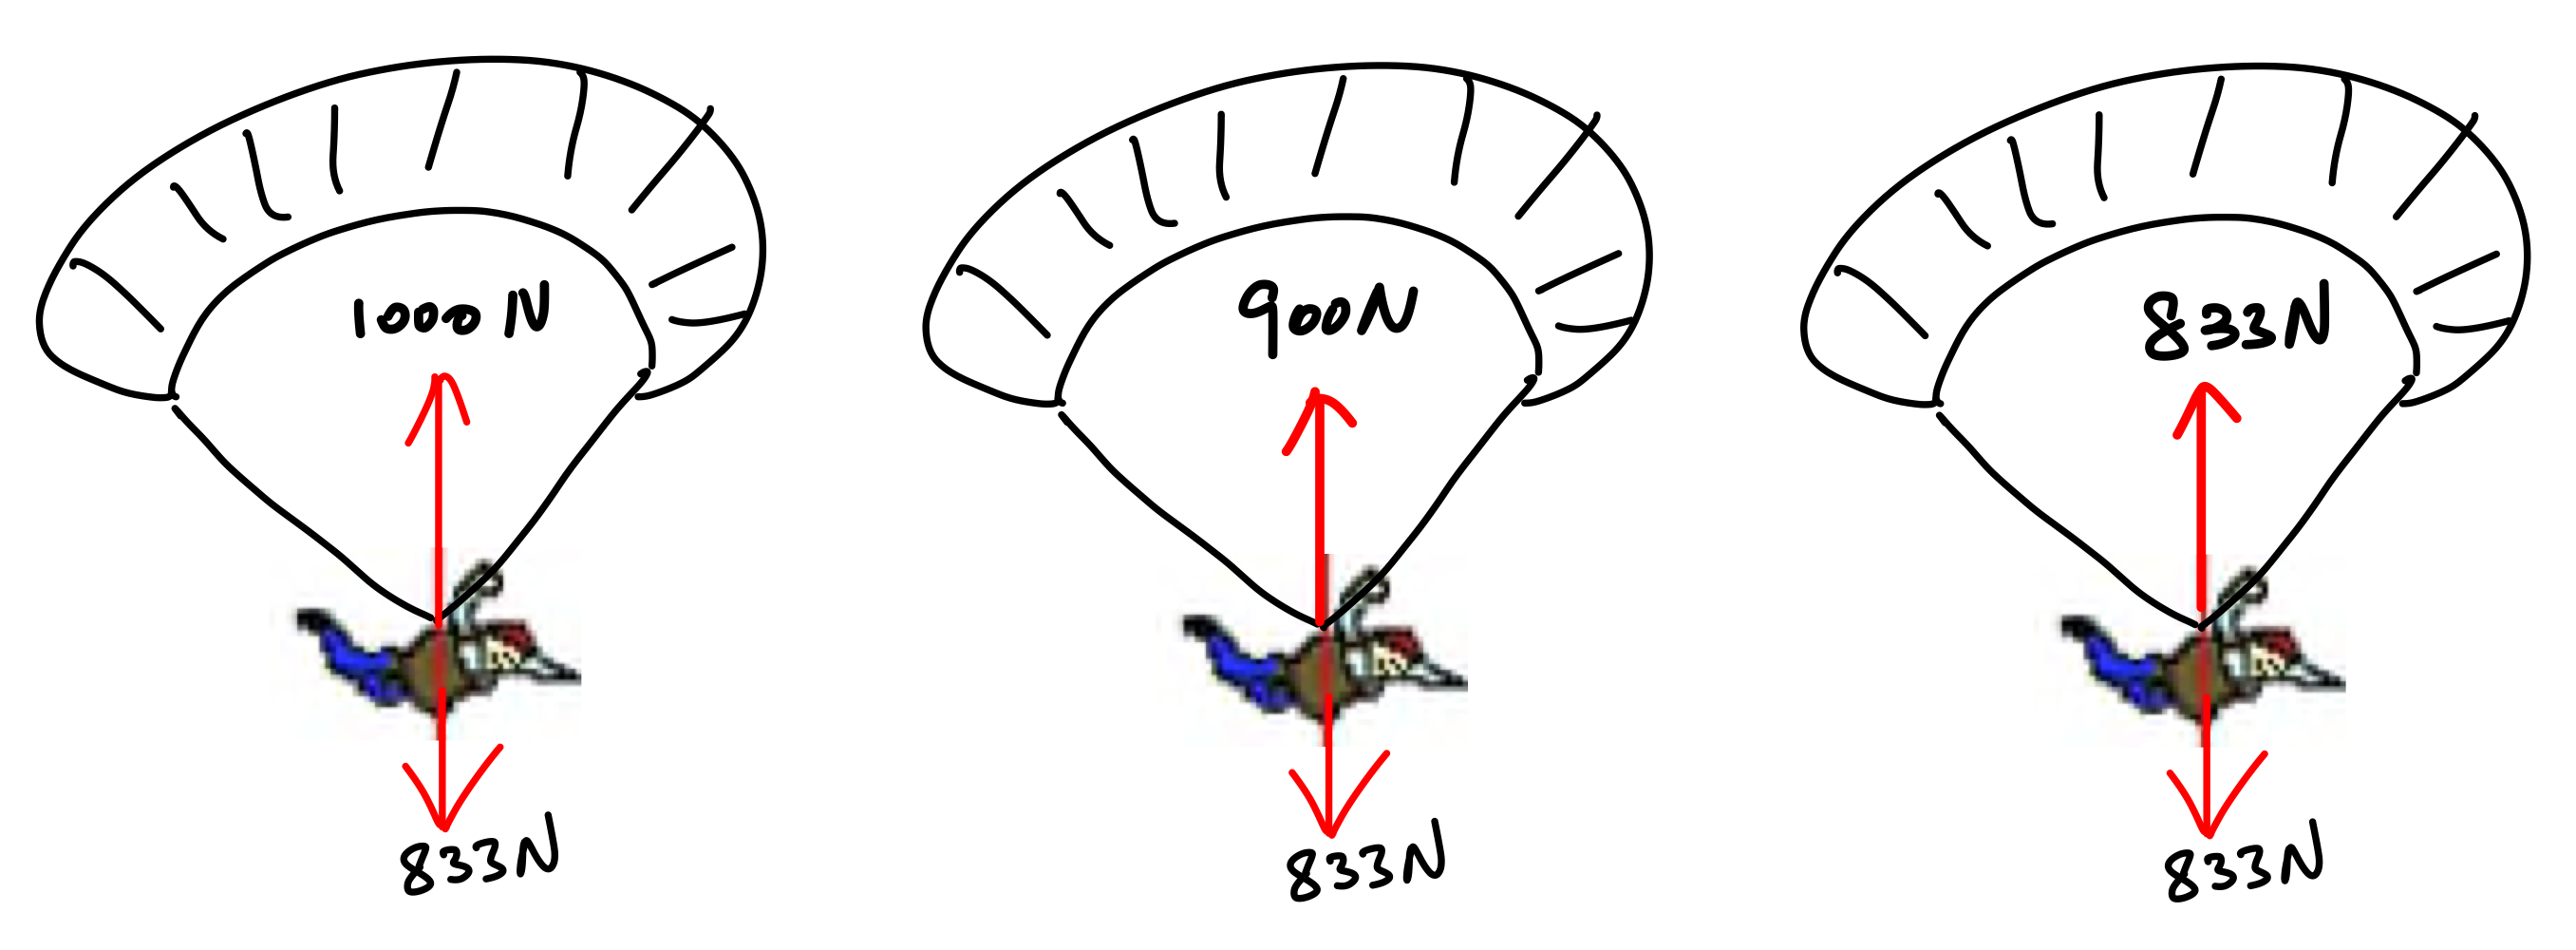
\includegraphics[width=.55\textwidth]{assets/bacb418f.png}
    \end{figure}

\end{frame}

\begin{frame}{流體阻力Fluid resistance}
    \begin{figure}[h!]
        \centering
        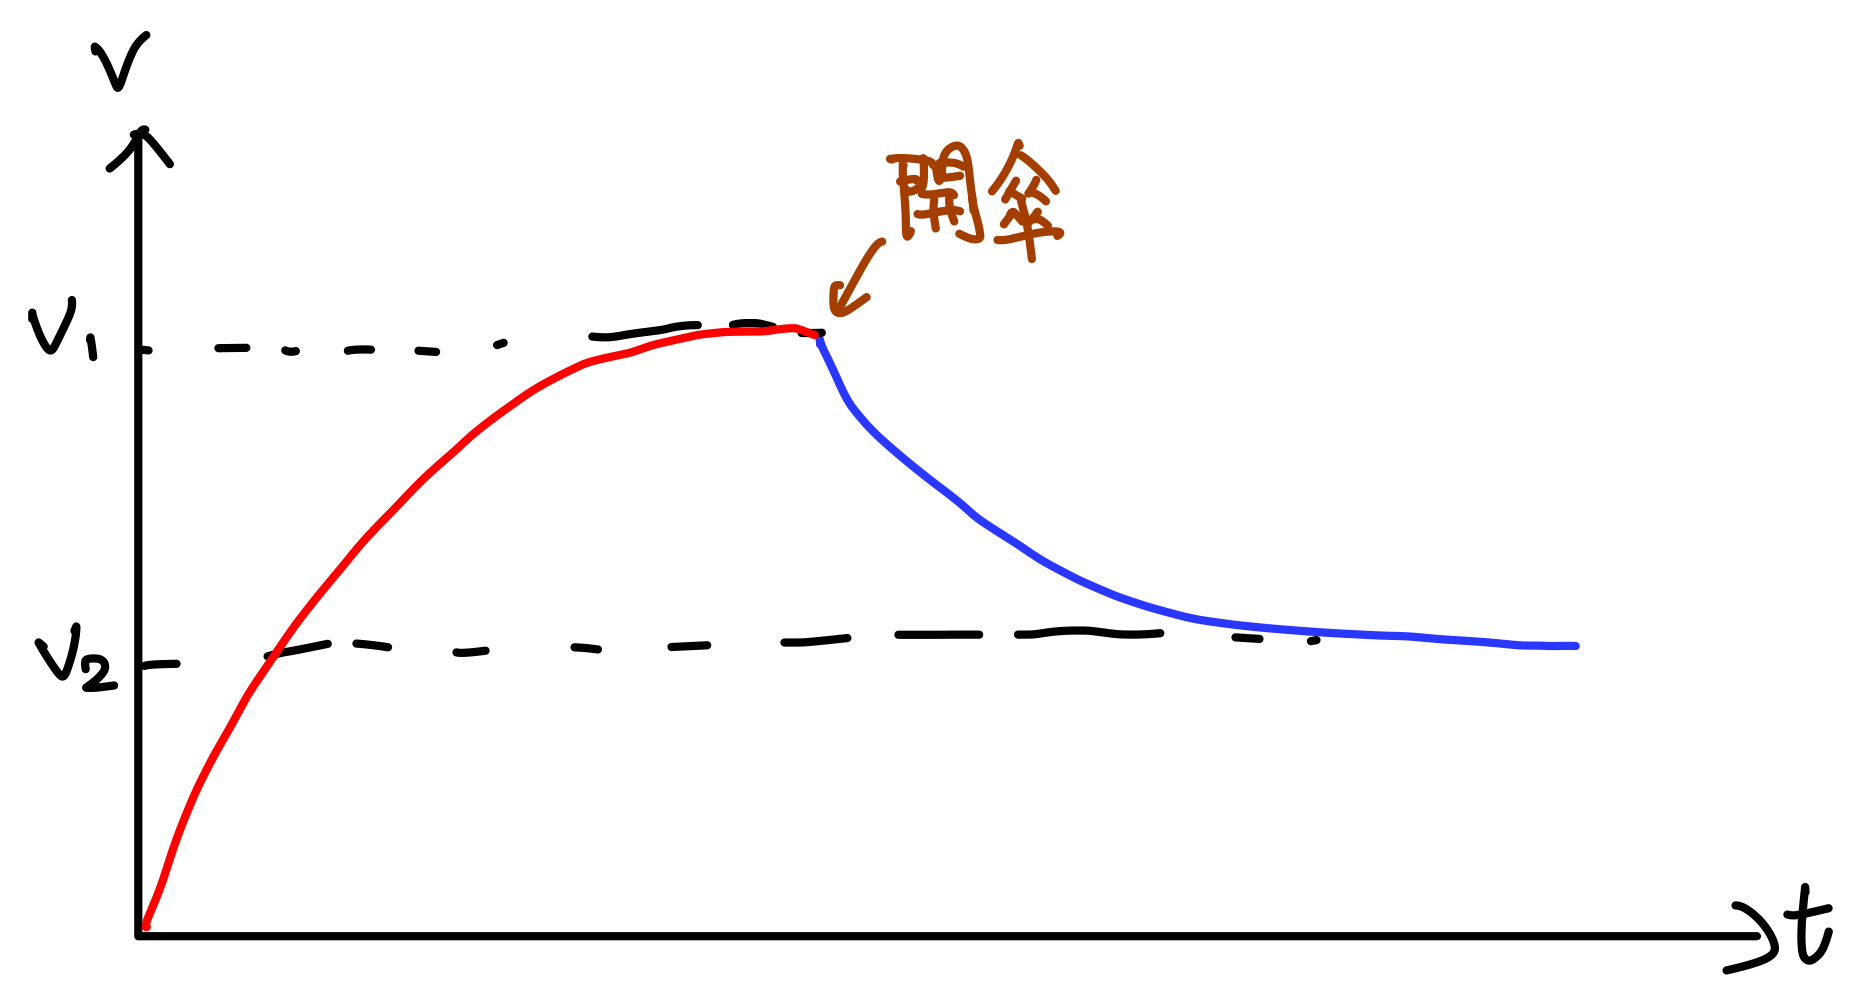
\includegraphics[width=.8\textwidth]{assets/7930445f.png}
        \caption{跳傘員的v-t線圖v-t graph of a falling skydiver}
    \end{figure}
\end{frame}
\begin{frame}{For interested students...}
    \begin{figure}[h!]
        \centering
        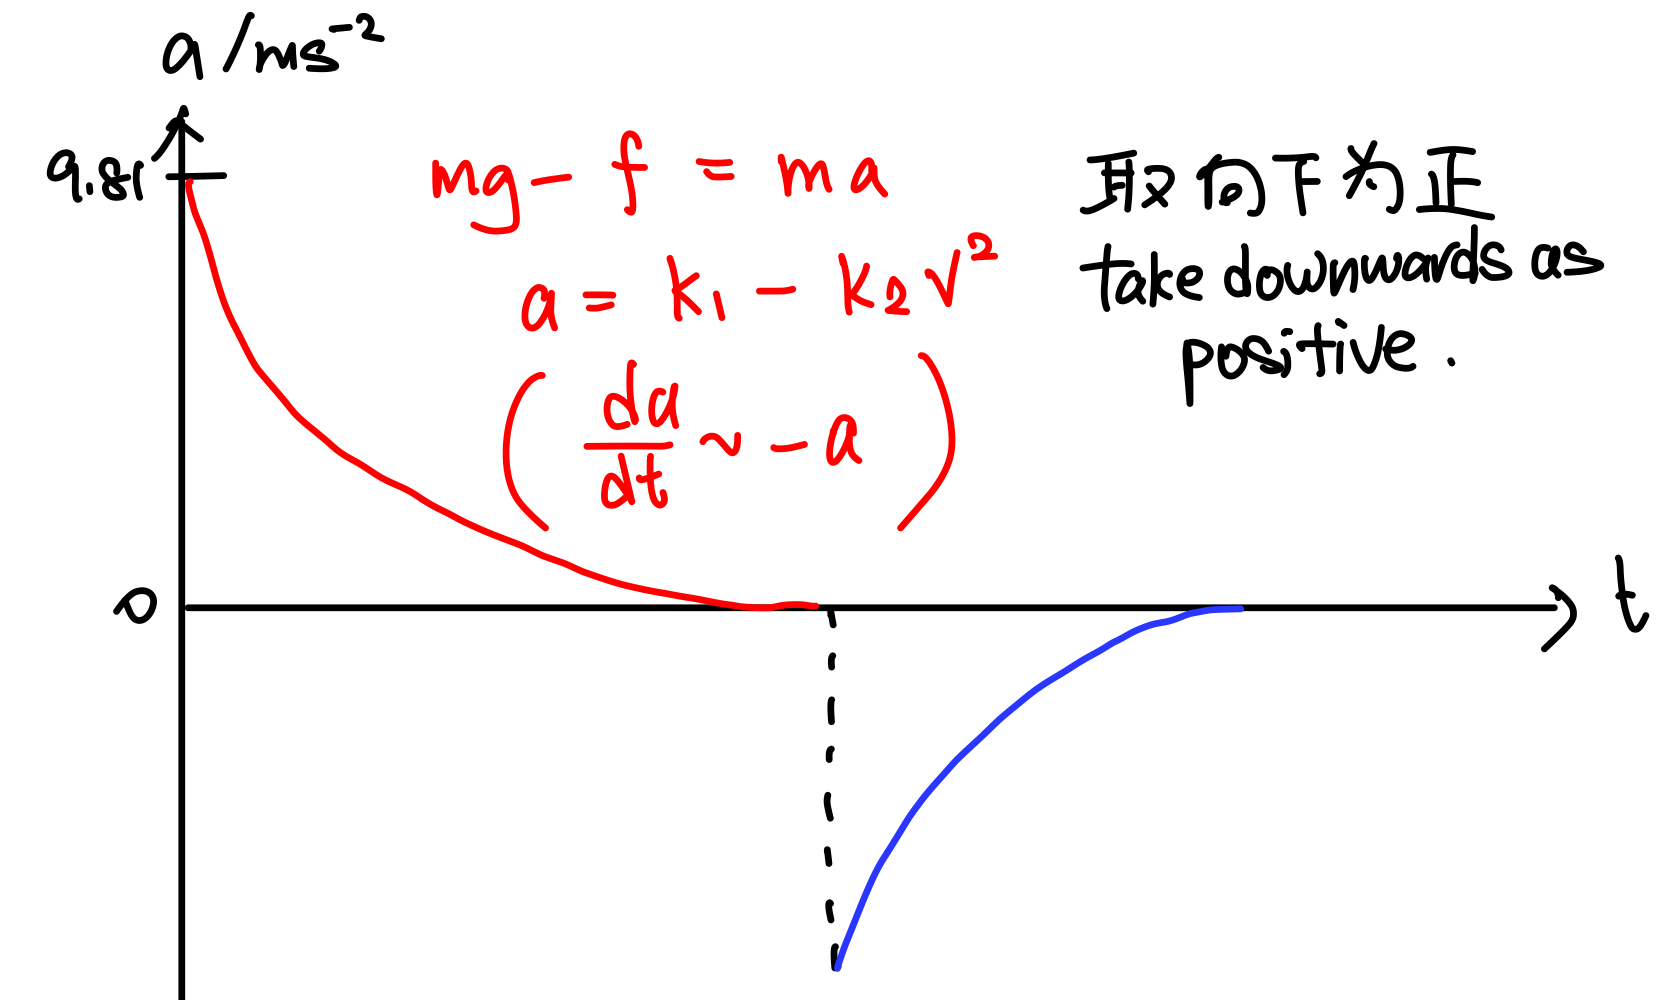
\includegraphics[width=0.55\textwidth]{assets/eda84940.png}
    \end{figure}
    \begin{figure}[h!]
        \centering
        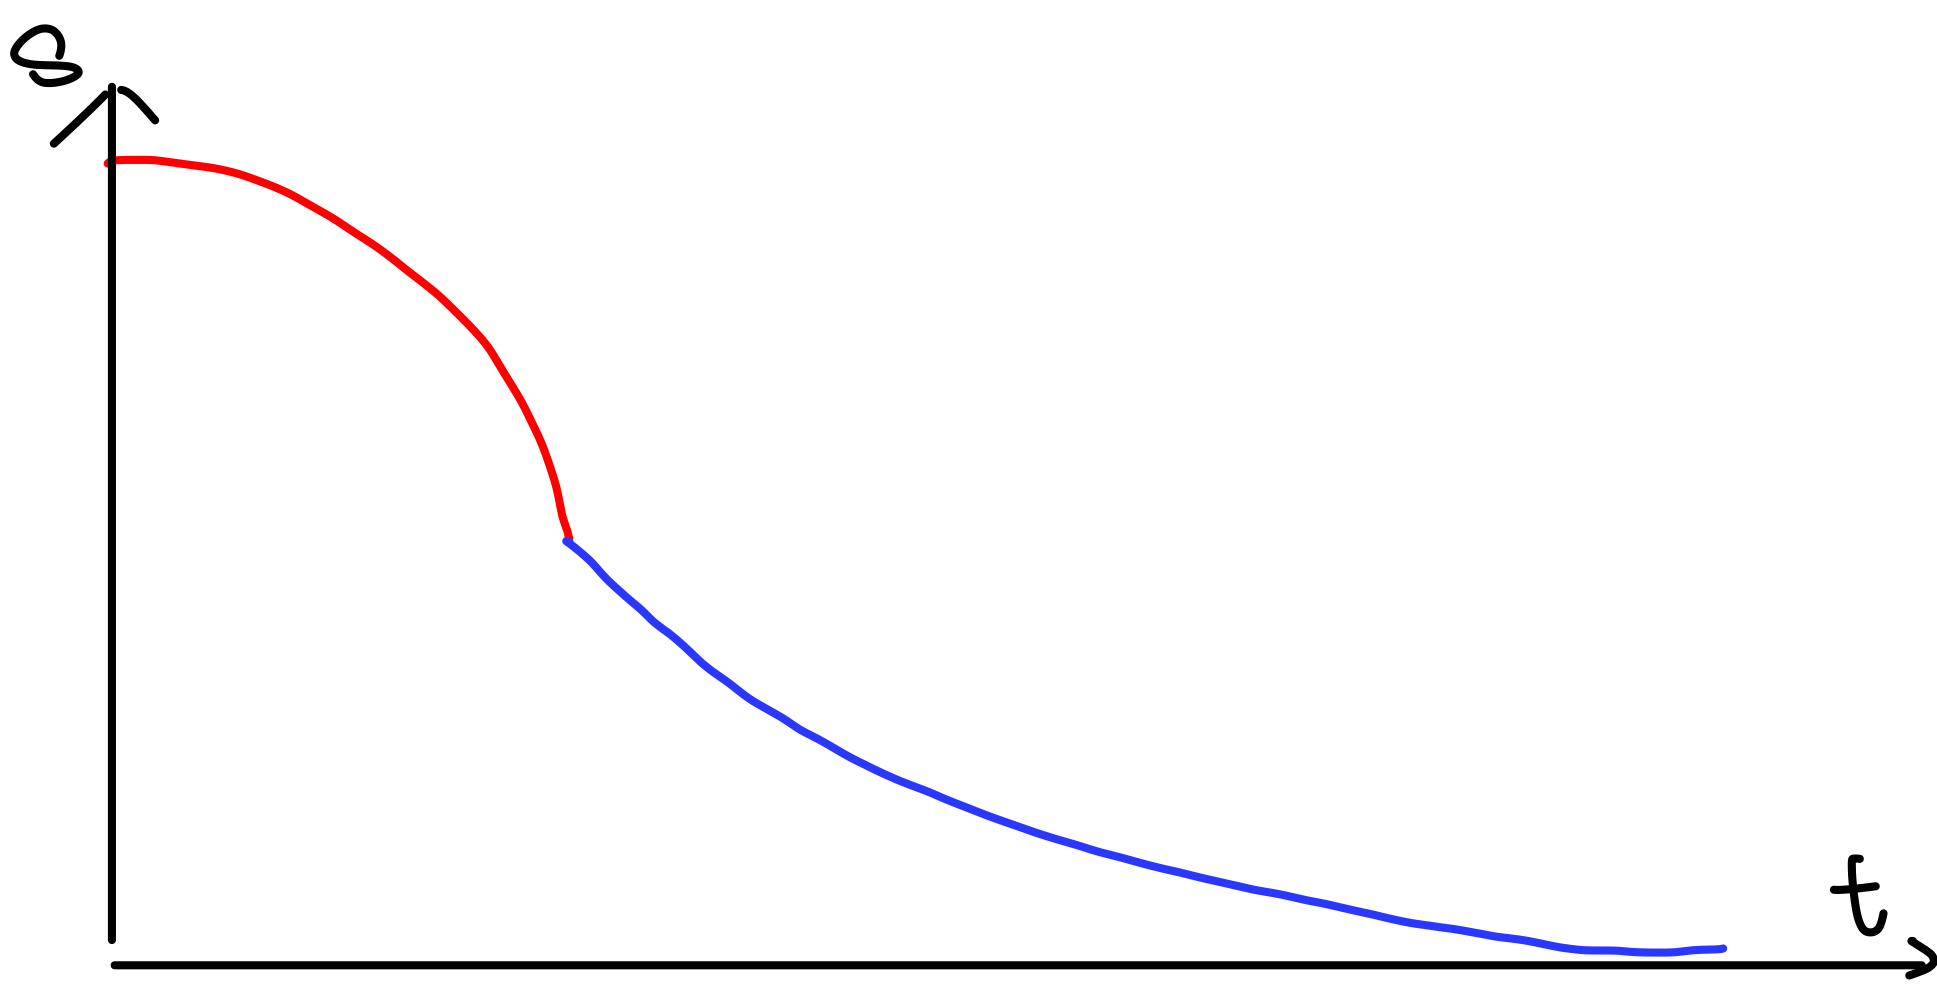
\includegraphics[width=0.55\textwidth]{assets/6689e5f4.png}
    \end{figure}
\end{frame}

\begin{frame}{牛頓第三定律 Newton's third law}
    \begin{exampleblock}
        {牛頓第三定律 Newton's third law}
        力總是成對出現。這些成對的力稱為作用力–反作用力對。 \\Forces always appear as pairs. These force pairs are known as action-reaction pairs.
    \end{exampleblock}\bigskip
    \begin{figure}[h!]
        \centering
        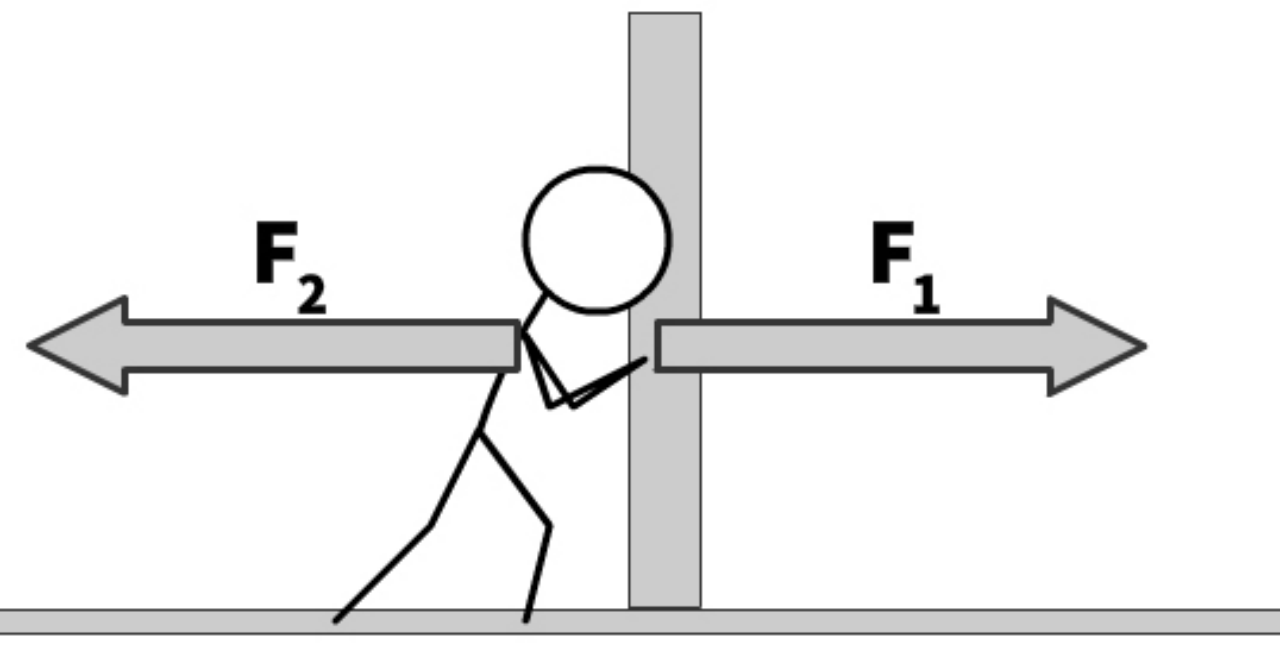
\includegraphics[width=.5\textwidth]{assets/350b642d.png}
    \end{figure}
\end{frame}
\begin{frame}{牛頓第三定律 Newton's third law}
    \begin{itemize}
        \item 作用力和反作用力的特性:\\Properties of action and reaction forces:
              \begin{itemize}
                  \item 量值相同same magnitudes
                  \item 方向相反different directions
                  \item 作用於不同的物體acting on different bodies
                  \item 必須屬於同一種力same type of force
              \end{itemize}
    \end{itemize}
\end{frame}
\begin{frame}{牛頓第三定律 Newton's third law}
    重量Weight:
    \begin{figure}[h!]
        \centering
        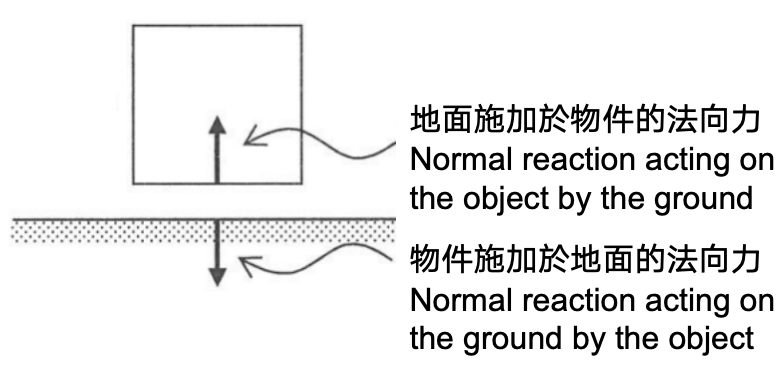
\includegraphics[width=.8\textwidth]{assets/4949a09b.png}
    \end{figure}
\end{frame}
\begin{frame}{牛頓第三定律 Newton's third law}
    法向力Normal reaction:
    \begin{figure}[h!]
        \centering
        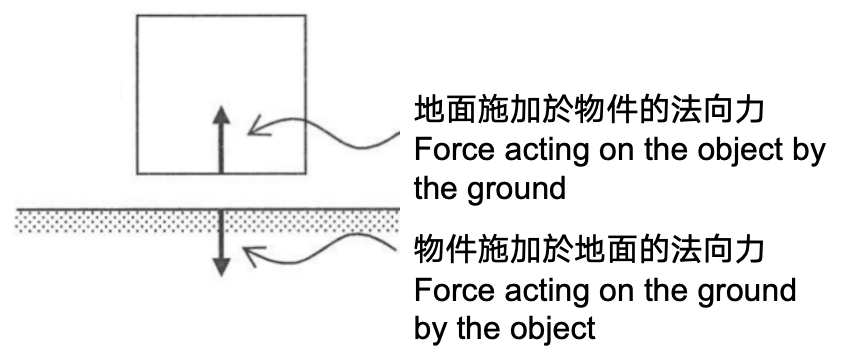
\includegraphics[width=.8\textwidth]{assets/69c3d3bd.png}
    \end{figure}
\end{frame}
\begin{frame}{牛頓第三定律 Newton's third law}
    張力Tension:
    \begin{figure}[h!]
        \centering
        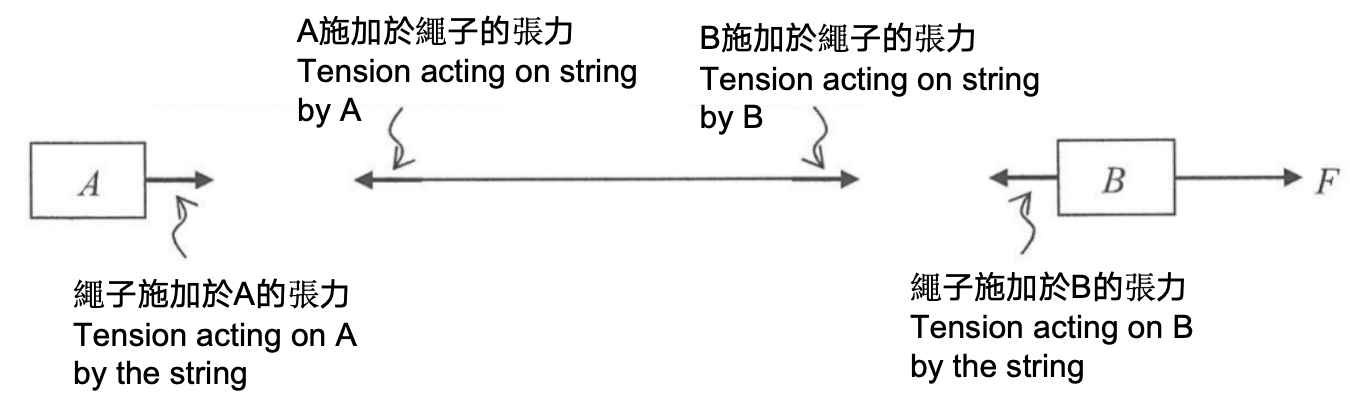
\includegraphics[width=.8\textwidth]{assets/f559bb67.png}
    \end{figure}
\end{frame}


\begin{frame}{牛頓第三定律 Newton's third law}
    \begin{figure}[h!]
        \centering
        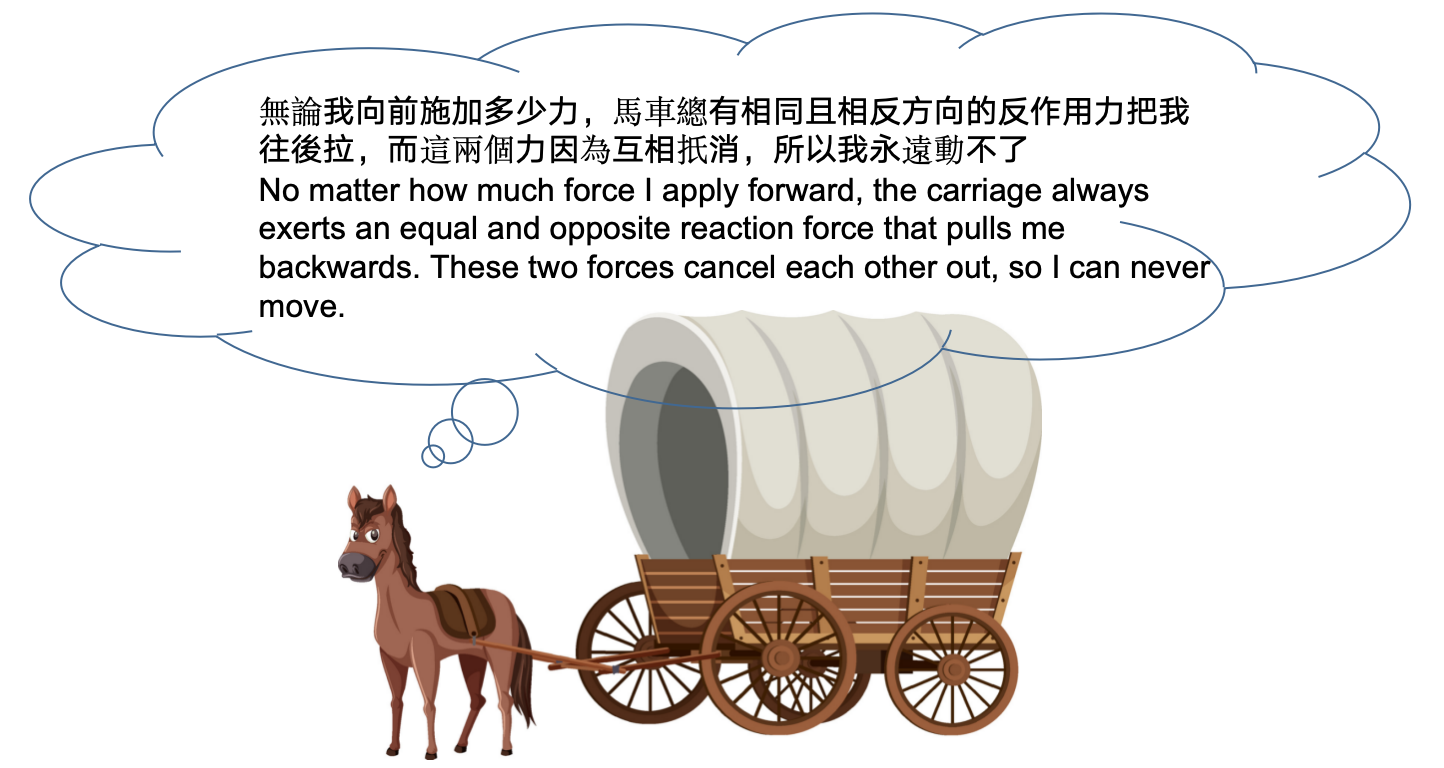
\includegraphics[width=\textwidth]{assets/4b5ef98a.png}
    \end{figure}
\end{frame}
\begin{frame}{牛頓第三定律 Newton's third law}
    \begin{figure}[h!]
        \centering
        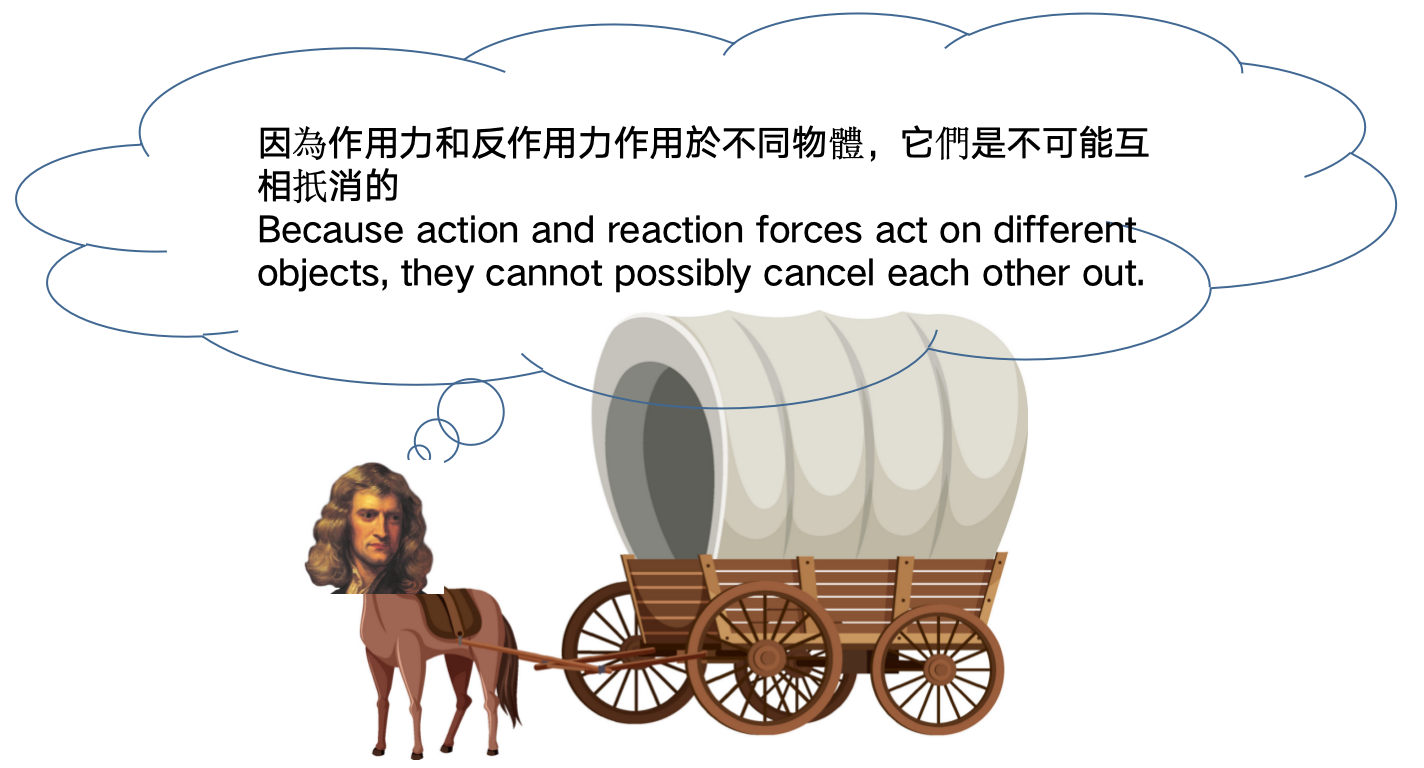
\includegraphics[width=\textwidth]{assets/9334d132.png}
    \end{figure}
\end{frame}

\begin{frame}{}
    \begin{figure}[h!]
        \centering
        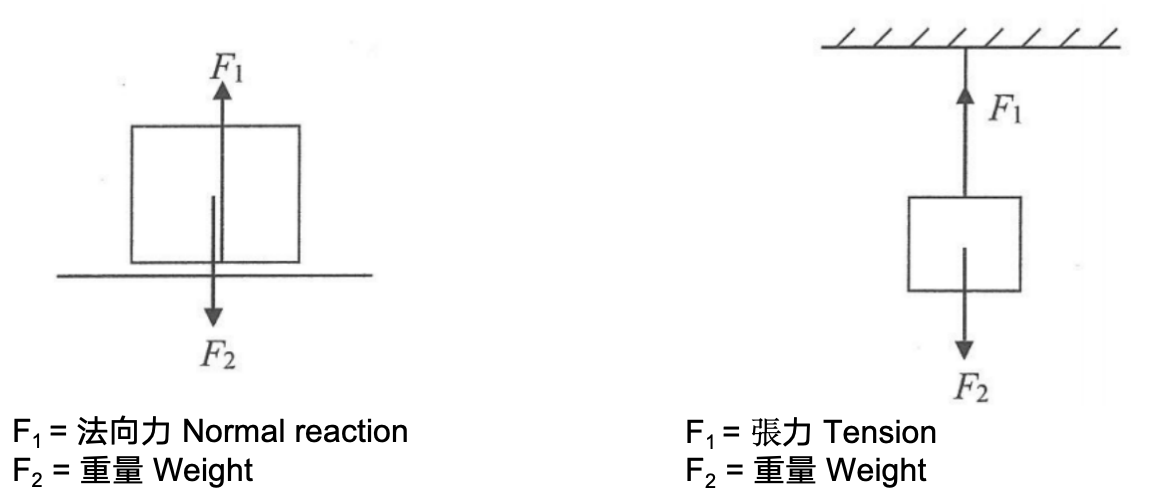
\includegraphics[width=.8\textwidth]{assets/6a71f82b.png}
    \end{figure}
    \begin{itemize}
        \item F$_1$ 和 F$_2$ 不是作用力反作用力對的理由:\\Reasons why F$_1$ and F$_2$ are not action reaction pair:
              \begin{itemize}
                  \item 作用於相同物體 Act on same object
                  \item 屬於不同種力 Different types of forces
              \end{itemize}
    \end{itemize}
\end{frame}



\begin{eg}
    \begin{figure}[h!]
        \centering
        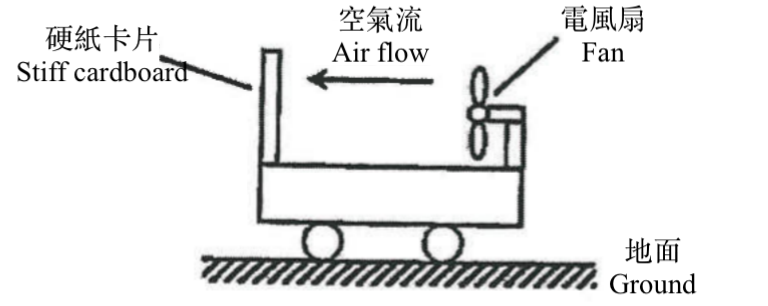
\includegraphics[width=0.66\textwidth]{assets/323c58f6.png}
    \end{figure}
    在小車的一端裝了電風扇,一張硬紙卡片固定在另一端且面向電風扇。當電風扇啓動後,小車將會怎樣運動?\\(a)不動(b)向左走(c)向右走(d)在原地往返運動
    \\An electric fan is installed on one end of the small car, and a stiff cardboard is fixed on the other end of the fan. When the electric fan is activated, how will the car move? \\(a) Remain at rest (b) Move left (c) Move right (d) Move left and right periodically

\end{eg}

\begin{eg}
    \begin{figure}[h!]
        \centering
        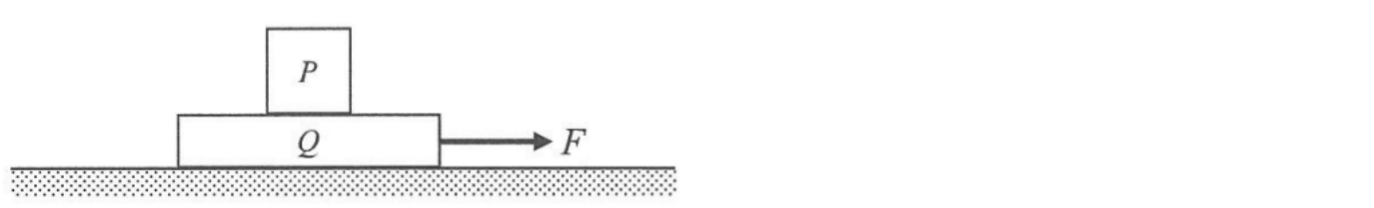
\includegraphics[width=.8\textwidth]{assets/9c913c73.png}
    \end{figure}
    P是 2kg,Q是 3kg,F 是 6N,所有接觸面都是光滑的。求P、Q的加速度。\\P is 2kg, Q is 3kg, F is 6N, and all contact surfaces are smooth.  Calculate the acceleration of P and Q.
\end{eg}

\begin{eg}
    \begin{figure}[h!]
        \centering
        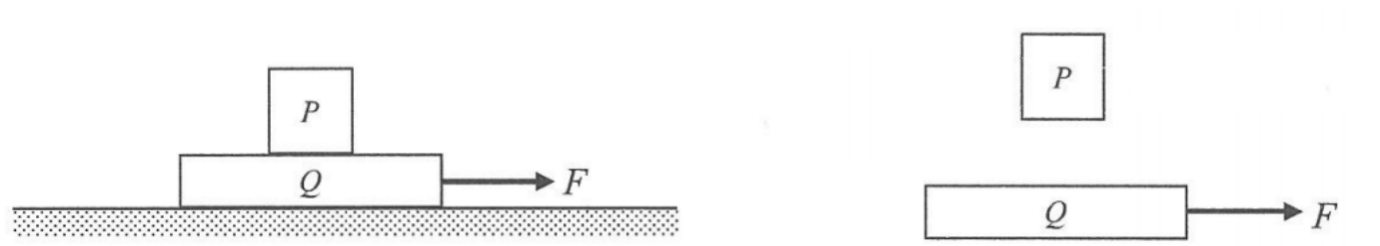
\includegraphics[width=.8\textwidth]{assets/5c3215d2.png}
    \end{figure}
    P是2kg,Q是3kg,F是6N,現在地面仍是光滑的,但P和Q之間存在摩擦力,使得P和Q能同時移動。求摩擦力的量值。\\P is 2kg, Q is 3kg, and F is 6N. The ground is still smooth, but there is friction between P and Q which allows them to move together. Calculate the magnitude of the frictional force.
\end{eg}

\begin{frame}{作用力和反作用力的日常應用Daily application of action and reaction pair}
    \begin{figure}[h!]
        \centering
        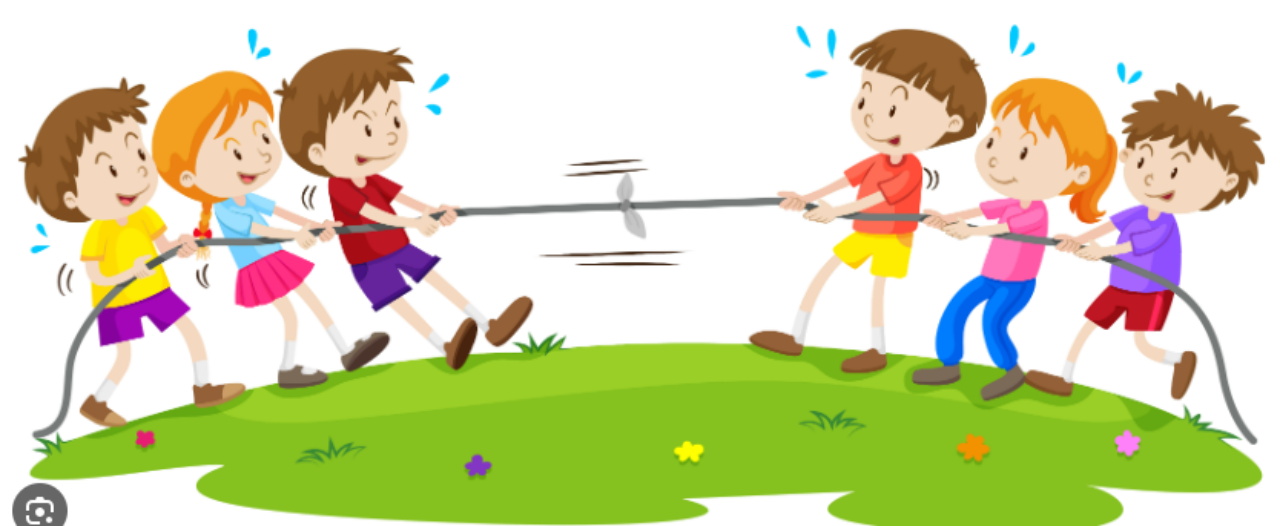
\includegraphics[width=.8\textwidth]{assets/ae0d3530.png}
    \end{figure}
    \begin{itemize}\bigskip
        \item 與地面產生的摩擦力大者勝出。\\Whichever side has greater friction on the ground wins.
    \end{itemize}
\end{frame}
\begin{frame}{作用力和反作用力的日常應用Daily application of action and reaction pair}
    \begin{figure}[h!]
        \centering
        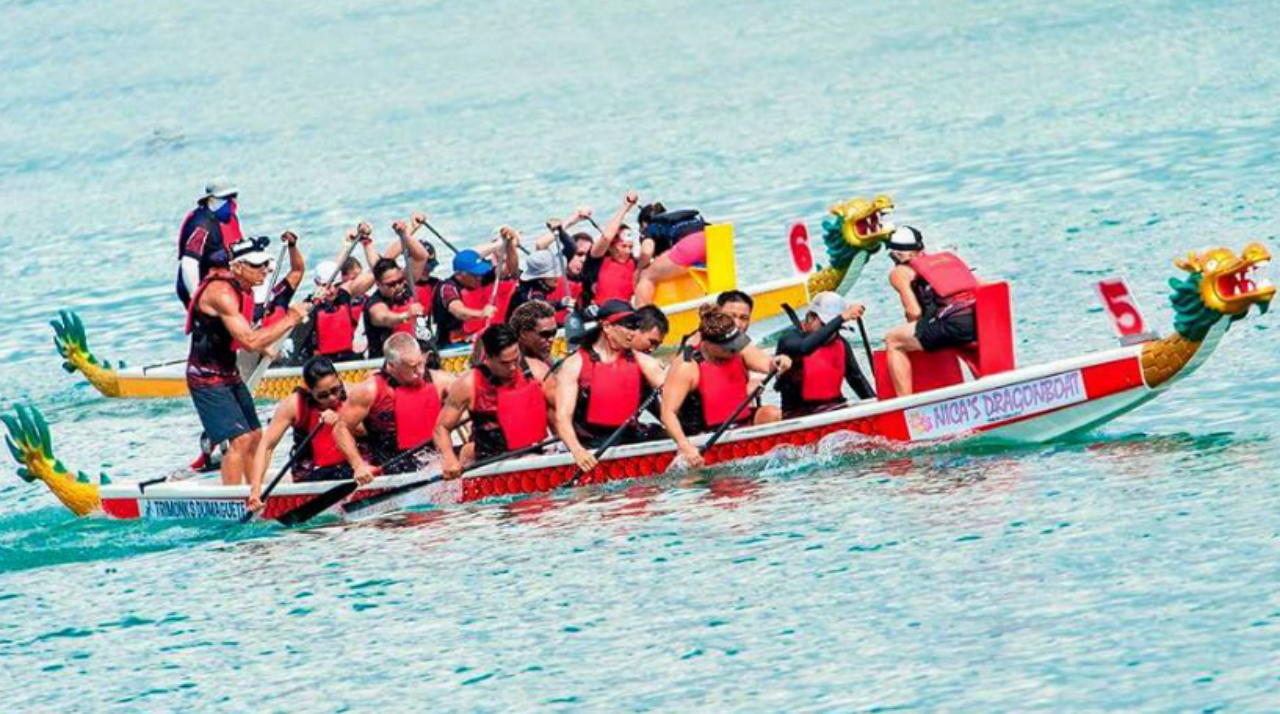
\includegraphics[width=.75\textwidth]{assets/45e1912d.png}
    \end{figure}
    \begin{itemize}
        \item 船槳向後推動河水,河水對船槳施加反作用力使船前進。\\The oar exert backward force on the river water, and the river water exerts a reaction force on the oar, causing the boat to move forward.
    \end{itemize}
\end{frame}
\begin{frame}{作用力和反作用力的日常應用Daily application of action and reaction pair}
    \begin{figure}[h!]
        \centering
        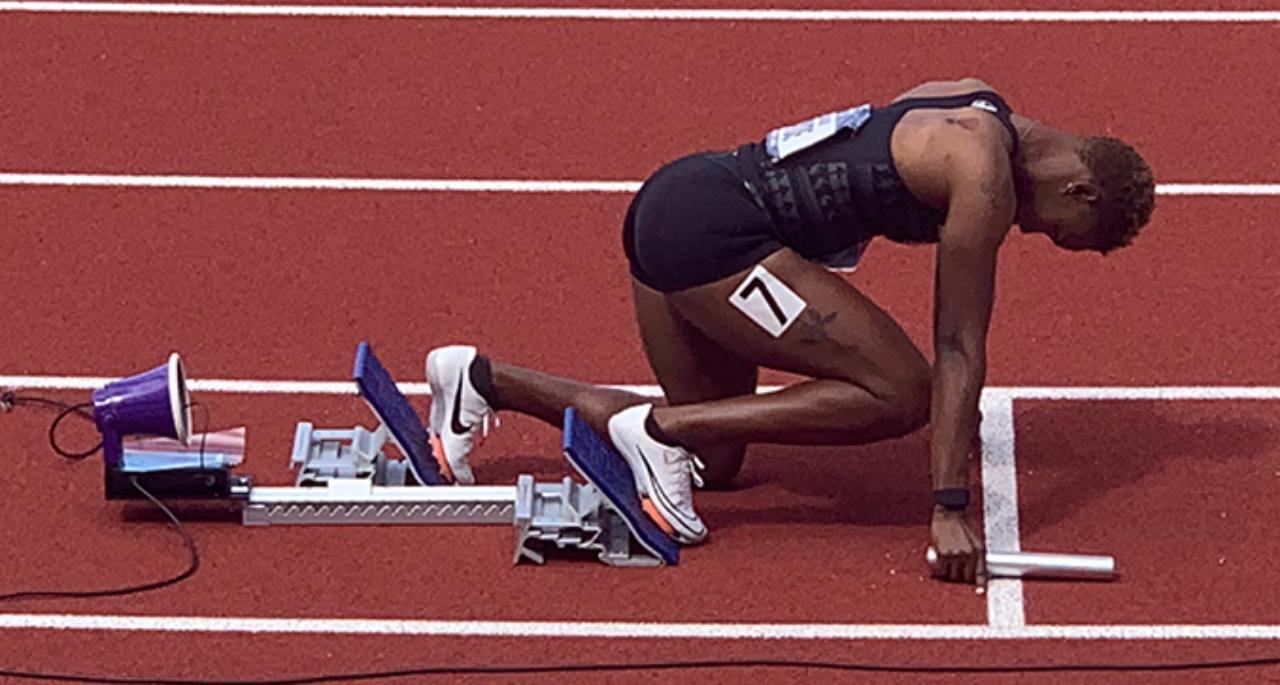
\includegraphics[width=.8\textwidth]{assets/60a0e41a.png}
    \end{figure}
    \begin{itemize}
        \item 助跑器為運動員在比賽開始時提供穩定且有爆發力的推動。\\Starting block is used to provide a stable and explosive push-off for athletes at the start of a race.
    \end{itemize}
\end{frame}
\end{document}